%%%%%%%%%%%%%%%%%%%%%%%%%%%%%%%%%%%%%%%%%%%%%%%%%%%%%%%%%%%%%%%%%%%%%%%%%%%%%%%%
%
% Template license:
% CC BY-NC-SA 3.0 (http://creativecommons.org/licenses/by-nc-sa/3.0/)
%
%%%%%%%%%%%%%%%%%%%%%%%%%%%%%%%%%%%%%%%%%%%%%%%%%%%%%%%%%%%%%%%%%%%%%%%%%%%%%%%%

%----------------------------------------------------------------------------------------
%	PACKAGES AND OTHER DOCUMENT CONFIGURATIONS
%----------------------------------------------------------------------------------------

\documentclass[
11pt, % The default document font size, options: 10pt, 11pt, 12pt
%oneside, % Two side (alternating margins) for binding by default, uncomment to switch to one side
%chapterinoneline,% Have the chapter title next to the number in one single line
spanish,
singlespacing, % Single line spacing, alternatives: onehalfspacing or doublespacing
%draft, % Uncomment to enable draft mode (no pictures, no links, overfull hboxes indicated)
%nolistspacing, % If the document is onehalfspacing or doublespacing, uncomment this to set spacing in lists to single
%liststotoc, % Uncomment to add the list of figures/tables/etc to the table of contents
%toctotoc, % Uncomment to add the main table of contents to the table of contents
parskip, % Uncomment to add space between paragraphs
%codirector, % Uncomment to add a codirector to the title page
headsepline, % Uncomment to get a line under the header
]{MastersDoctoralThesis} % The class file specifying the document structure



%----------------------------------------------------------------------------------------
%	INFORMACIÓN DE LA MEMORIA
%----------------------------------------------------------------------------------------

\thesistitle{Predicción de eventos graves en pacientes hipertensos basado en informes de presurometrías a partir de la aplicación de técnicas de
inteligencia artificial} % El títulos de la memoria, se usa en la carátula y se puede usar el cualquier lugar del documento con el comando \ttitle

% Nombre del posgrado, se usa en la carátula y se puede usar el cualquier lugar del documento con el comando \degreename
%\posgrado{Carrera de Especialización en Sistemas Embebidos} 
%\posgrado{Carrera de Especialización en Internet de las Cosas} 
\posgrado{Carrera de Especialización en Intelegencia Artificial}
%\posgrado{Maestría en Sistemas Embebidos} 
%\posgrado{Maestría en Internet de las cosas}

\author{Ing. Trinidad Monreal} % Tu nombre, se usa en la carátula y se puede usar el cualquier lugar del documento con el comando \authorname

\director{Dr. Ing. Roberto A. Bunge (UdeSA)} % El nombre del director, se usa en la carátula y se puede usar el cualquier lugar del documento con el comando \dirname
%\codirector{Nombre del codirector (pertenencia)} % El nombre del codirector si lo hubiera, se usa en la carátula y se puede usar el cualquier lugar del documento con el comando \codirname.  Para activar este campo se debe descomentar la opción "codirector" en el comando \documentclass, línea 23.

\juradoUNO{Nombre del jurado 1 (pertenencia)} % Nombre y pertenencia del un jurado se usa en la carátula y se puede usar el cualquier lugar del documento con el comando \jur1name
\juradoDOS{Nombre del jurado 2 (pertenencia)} % Nombre y pertenencia del un jurado se usa en la carátula y se puede usar el cualquier lugar del documento con el comando \jur2name
\juradoTRES{Nombre del jurado 3 (pertenencia)} % Nombre y pertenencia del un jurado se usa en la carátula y se puede usar el cualquier lugar del documento con el comando \jur3name

%\ciudad{Ciudad Autónoma de Buenos Aires}
\ciudad{Ciudad Autónoma de Buenos Aires}

\fechaINICIO{octubre de 2022}
\fechaFINAL{agosto de 2023}


\keywords{inteligencia artificial, FIUBA} % Keywords for your thesis, print it elsewhere with \keywordnames
\usepackage{hyperref}
\usepackage{amsfonts}
\usepackage{nicefrac}
\usepackage{amsmath}
\usepackage{algorithm}
\usepackage{algpseudocode}


\begin{document}


\frontmatter % Use roman page numbering style (i, ii, iii, iv...) for the pre-content pages

\pagestyle{plain} % Default to the plain heading style until the thesis style is called for the body content


%----------------------------------------------------------------------------------------
%	RESUMEN - ABSTRACT 
%----------------------------------------------------------------------------------------

\begin{abstract}
\addchaptertocentry{\abstractname} % Add the abstract to the table of contents
%
%The Thesis Abstract is written here (and usually kept to just this page). The page is kept centered vertically so can expand into the blank space above the title too\ldots
\centering

%El resumen debe escribirse en uno o dos párrafo.  Debe ser breve y conciso sin ningún elemento de formato en el texto como itálicas o negrita. Tampoco se deben usar siglas ni acrónimos que no resulten obvios para un lector promedio de la memoria, ni referencias bibliográficas o notas al pie de página.  No debe faltar qué es lo que se hizo/logró, qué importancia/valor tiene el proyecto/resultado, qué va a encontrar el lector en la memoria y qué contenidos de la especialización/maestría se aplicaron en el proyecto.
En esta memoria se describe el diseño y la implementación de un software de inteligencia artificial desarrollado para el Hospital Alemán. El modelo utiliza datos obtenidos de presurometrías realizadas a pacientes hipertensos, con el propósito de predecir el riesgo de sufrir eventos cardiovasculares graves. Como resultado, este trabajo permite al servicio de cardiología e hipertensión definir estrategias de tratamiento personalizadas para cada grupo de riesgo.

Para llevar a cabo este trabajo se emplearon técnicas de estadística, análisis de datos y criterios de selección de características, así como modelos de aprendizaje profundo para lograr la clasificación.

\end{abstract}

%----------------------------------------------------------------------------------------
%	CONTENIDO DE LA MEMORIA  - AGRADECIMIENTOS
%----------------------------------------------------------------------------------------

%\begin{acknowledgements}
%\addchaptertocentry{\acknowledgementname} % Descomentando esta línea se puede agregar los agradecimientos al índice
%\vspace{1.5cm}

%Esta sección es para agradecimientos personales y es totalmente \textbf{OPCIONAL}.  

%\end{acknowledgements}

%----------------------------------------------------------------------------------------
%	LISTA DE CONTENIDOS/FIGURAS/TABLAS
%----------------------------------------------------------------------------------------

\tableofcontents % Prints the main table of contents

\listoffigures % Prints the list of figures

\listoftables % Prints the list of tables


%----------------------------------------------------------------------------------------
%	CONTENIDO DE LA MEMORIA  - DEDICATORIA
%----------------------------------------------------------------------------------------

%\dedicatory{\textbf{Dedicado a... [OPCIONAL]}}  % escribir acá si se desea una dedicatoria

%----------------------------------------------------------------------------------------
%	CONTENIDO DE LA MEMORIA  - CAPÍTULOS
%----------------------------------------------------------------------------------------

\mainmatter % Begin numeric (1,2,3...) page numbering

\pagestyle{thesis} % Return the page headers back to the "thesis" style

% Incluir los capítulos como archivos separados desde la carpeta Chapters

% Chapter 1

\chapter{Introducción general} % Main chapter title

\label{Chapter1} % For referencing the chapter elsewhere, use \ref{Chapter1} 
\label{IntroGeneral}

%----------------------------------------------------------------------------------------

% Define some commands to keep the formatting separated from the content 
\newcommand{\keyword}[1]{\textbf{#1}}
\newcommand{\tabhead}[1]{\textbf{#1}}
\newcommand{\code}[1]{\texttt{#1}}
\newcommand{\file}[1]{\texttt{\bfseries#1}}
\newcommand{\option}[1]{\texttt{\itshape#1}}
\newcommand{\grados}{$^{\circ}$}

%----------------------------------------------------------------------------------------

%\section{Introducción}

%----------------------------------------------------------------------------------------
% 1.1(5 hojas)---------------------------------------------------------------------------
%----------------------------------------------------------------------------------------
\section{Conceptos básicos de la presión arterial y sus métodos de medición}

En esta sección, se abordará la definición de la presión arterial normal y la hipertensión, 
así como el uso de las presurometrías como herramienta complementaria en su diagnóstico y seguimiento.

\subsection{Presión arterial normal e hipertensión arterial}

La presión arterial (PA) es la fuerza por unidad de superficie ejercida por la sangre contra las paredes 
de las arterias \citep{CITE:1}. Sin profundizar en los principios físicos, parece relevante destacar que el corazón 
bombea la sangre de forma pulsátil. Por este motivo, la PA alterna entre una presión arterial sistólica (PAS) 
y una presión arterial diastólica (PAD). En la figura \ref{fig:aorticPulse} se expone un registro típico de las pulsaciones 
de la presión en la raíz de la arteria aorta \citep{CITE:2} \citep{CITE:3}. 

\begin{figure}[h]
  \centering
  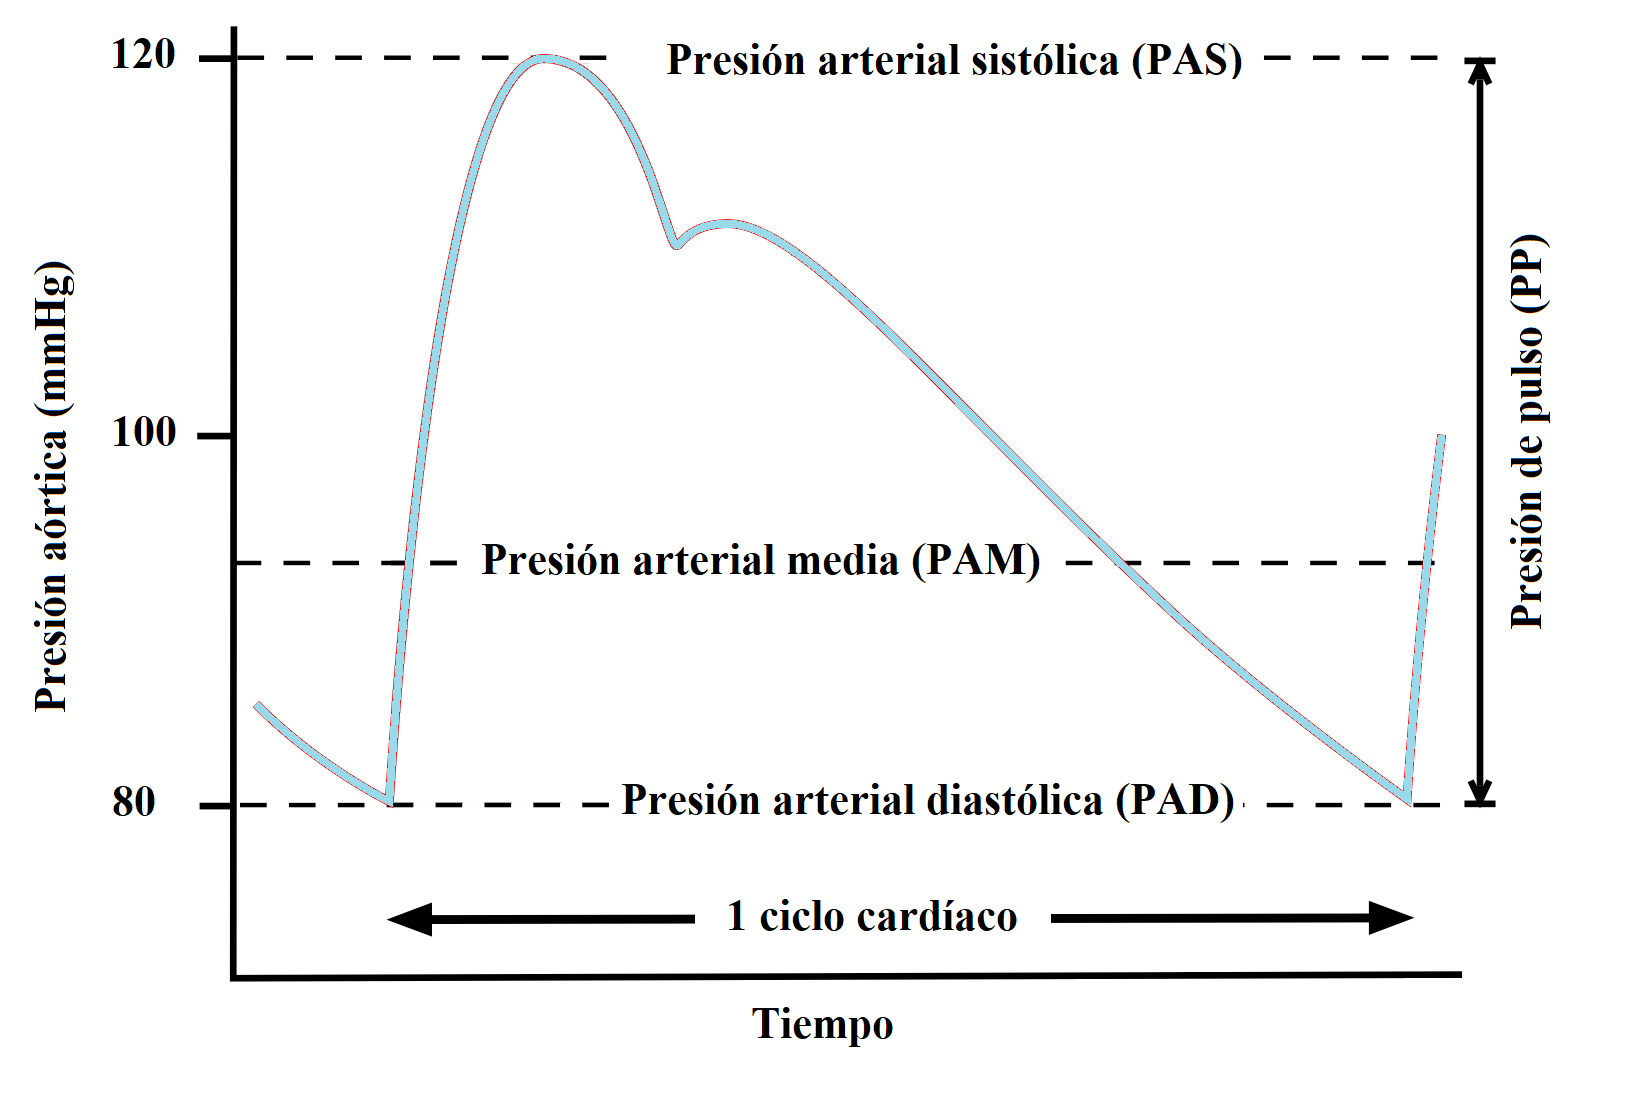
\includegraphics[width=\textwidth]{./Figures/aortic-pulse-pressure.png}
  \caption{Representación esquemática del pulso de presión registrado en la aorta ascendente.\protect\footnotemark.}\label{fig:aorticPulse}
\end{figure}

\footnotetext{Imagen adaptada de Klabunde, R. E. (2013). Normal and Abnormal Blood Pressure (Physiology, Pathophysiology and Treatment). Kindle Edition.}

En un adulto joven sano, la presión máxima o PAS es de 
120 mmHg y la presión mínima o PAD en cada pulso es de 80 mmHg. La diferencia entre estas dos presiones 
se conoce cómo la presión de pulso (PP) y ronda unos 40 mmHg. Por otro lado, la presión arterial media (PAM) 
está determinada en un 60\% por la PAD y en un 40\% por la PAS, dado que se invierte una mayor fracción 
del ciclo cardíaco en la diástole que en la sístole \citep{CITE:2} \citep{CITE:3}. Así, la expresión matemática que describe 
a la PAM es la siguiente: 

\begin{equation}
	\label{eq:PAM}
	PAM = \frac{(2*PAD + PAS)}{3}
\end{equation}

La PA alta o hipertensión arterial (HTA) es uno de los principales factores de riesgo para las enfermedades 
cardiovasculares, tales cómo la enfermedad cerebrovascular, insuficiencia cardíaca, cardiopatía isquémica, 
enfermedad renal terminal, arteriopatía periférica y retinopatía \citep{CITE:6} \citep{CITE:7}. Actualmente, se utiliza cómo guía 
la clasificación de HTA de la tabla \ref{tab:TablaHTA}.

\begin{table}[h]
	\centering
	\caption[Clasificación de la presión arterial por niveles]{Clasificación de la presión arterial por niveles.\protect\footnotemark.}
	\begin{tabular}{l c c c}    
		\toprule
		\textbf{Grado} 	      & \textbf{Presión arterial sistólica} 	& \textbf{}	& \textbf{Presión arterial diastólica}  \\
		\midrule
		Óptima                & <\ 120 mmHg                           & 	y			  & <\ 80 mmHg \\		
    Normal                & 120-129 mmHg                          &  	y/o			& 80-84 mmHg \\	
    Normal-alta           & 130-139 mmHg                          & 	y/o			& 85-89 mmHg \\	
    HTA de grado I        & 140-159 mmHg                          & 	y/o			& 90-99 mmHg \\
    HTA de grado II       & 160-179 mmHg                          & 	y/o			& 100-109 mmHg \\		
    HTA de grado III      & $\geq$  180 mmHg                      & 	y/o			& $\geq$  110 mmHg \\	
		\bottomrule
		\hline
	\end{tabular}
	\label{tab:TablaHTA}
\end{table}

\footnotetext{Tabla realizada con información de López Farré, A. y Macaya Miguel, C. (2009). Libro de la salud cardiovascular del hospital clínico San Carlos y la fundación BBVA (pp. 121-129). Editorial Nerea, S.A.}

\subsection{Presurometrías}

Las mediciones de PA en el consultorio médico son necesarias pero insuficientes para un adecuado diagnóstico, 
tratamiento y seguimiento de la HTA. El monitoreo ambulatorio de presión arterial (MAPA), también conocido 
como presurometría, es un examen complementario que permite evaluar la PA en el contexto de la vida cotidiana 
del paciente. A diferencia de las mediciones de PA en el consultorio, que se realizan en condiciones 
estandarizadas, el MAPA obtiene un gran número de mediciones a lo largo de un día habitual del paciente. 
Esto proporciona la capacidad de medir la tensión arterial durante el reposo, sueño, actividad física y mental, 
trabajo y período postprandial. Conocer la PA ambulatoria permite identificar diferentes patrones de HTA, tales 
como: HTA diurna, HTA nocturna, HTA durante todo el día, HTA durante el sueño e HTA de guardapolvo blanco 
(solo presente en el consultorio médico). Por lo tanto, este estudio puede ser un predictor más efectivo de 
la mortalidad y eventos cardiovasculares que simplemente basarse en la medición de la presión arterial en el 
consultorio médico \citep{CITE:7} \citep{CITE:5}.

Actualmente, el MAPA es el único método disponible para medir la PA durante la noche, y diversos estudios 
demuestran que la PA nocturna tiene un mayor valor pronóstico que la PA diurna. Por esta razón, se recomienda 
incluir el MAPA cómo parte del diagnóstico de la HTA. Es especialmente útil cuando los valores de PA en el 
consultorio se encuentran en un rango limítrofe (grado normal-alta según la tabla \ref{tab:TablaHTA}) en 
varias consultas consecutivas. Las indicaciones actuales para definir la HTA mediante el MAPA se detallan 
en la tabla \ref{tab:HTA-MAPA} \citep{CITE:7}.

\begin{table}[h]
	\centering
	\caption[Valores de referencia para definir HTA por MAPA]{Valores de referencia para definir HTA por MAPA.\protect\footnotemark.}
	\begin{tabular}{l c c c}    
		\toprule
		\textbf{} 	      & \textbf{Presión arterial sistólica} 	& \textbf{}	& \textbf{Presión arterial diastólica}  \\
		\midrule
    PA de 24 horas     &  $\geq$ 130 mmHg                     & 	y/o			&  $\geq$ 80 mmHg \\	
    PA diurna          &  $\geq$ 135 mmHg                     & 	y/o			&  $\geq$ 85 mmHg \\	
    PA nocturna        &  $\geq$ 120 mmHg                     & 	y/o			&  $\geq$ 70 mmHg \\	
		\bottomrule
		\hline
	\end{tabular}
	\label{tab:HTA-MAPA}
\end{table}

\footnotetext{Tabla realizada con información de Cuffaro, P. E., Morales, M. S. y Waisman, G. D. (2013). MONITOREO AMBULATORIO DE PRESIÓN ARTERIAL. En SAHA (Ed.), Hipertension Arterial, Epidemiología, Fisiología, Fisiopatología, Diagnóstico y Tratamiento. (pp. 391-395). Buenos Aires.}

El MAPA se lleva a cabo mediante dispositivos conocidos como presurómetros o \textit{holters} de presión arterial. 
Un técnico en cardiología coloca el presurómetro en el brazo del paciente, y se retira al día siguiente. 
El instrumento consiste en un manguito de presión arterial conectado a una grabadora, como se muestra en 
la figura \ref{fig:holter}. Esta realiza un inflado periódico cada 20 a 30 minutos, y los datos se almacenan en una memoria 
de estado sólido, generalmente en una tarjeta SD. Luego, los datos son analizados mediante el software del 
dispositivo \citep{CITE:3} \citep{CITE:7}.

\begin{figure}[h]
  \centering
  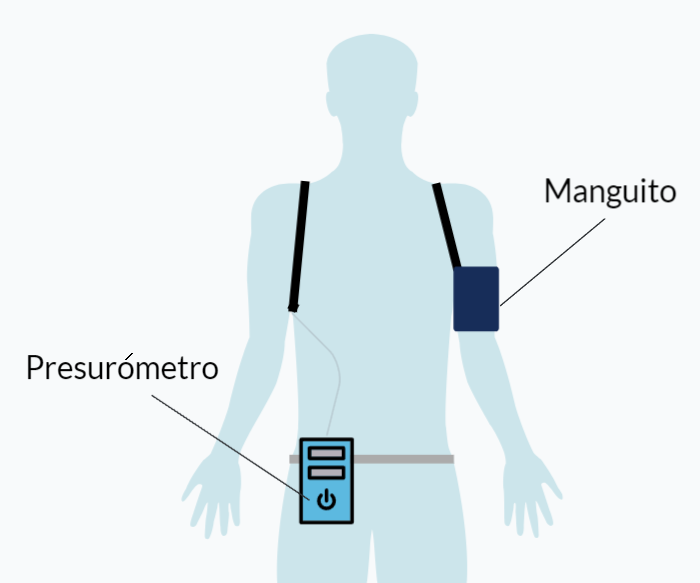
\includegraphics[width=.7\textwidth]{./Figures/presurometro.png}
  \caption{Esquema de un \textit{holter} de presión arterial.}
  \label{fig:holter}
\end{figure}


%----------------------------------------------------------------------------------------
% 1.2 (1 hoja)------------------------------------------------------------------------------------
%----------------------------------------------------------------------------------------
\section{Contexto y motivación}

La incorporación de técnicas de inteligencia artificial (IA) en la medicina cardiovascular es una de las principales 
motivaciones en la realización de este trabajo. A medida que la IA se desarrolla en distintos campos, su aplicación 
en el ámbito de la salud experimenta un crecimiento significativo. Sin embargo, uno de los desafíos clave que la IA 
enfrenta en la medicina es la limitación de datos disponibles para entrenar modelos de aprendizaje profundo \citep{CITE:8}.

En el caso particular del Hospital Alemán de Buenos Aires, el servicio de cardiología posee una gran cantidad de 
datos de informes de presurometrías de pacientes hipertensos. Aunque el personal carece de experiencia en herramientas 
de aprendizaje automático o aprendizaje profundo, los profesionales médicos comprenden el potencial de estos datos de 
MAPA para facilitar la identificación de patrones, factores de riesgo y respuestas al tratamiento de HTA. Además, 
es importante destacar que este trabajo se alinea con la misión del Hospital Alemán, que busca la actualización constante 
de tecnologías para garantizar una mejor atención médica basada en la investigación \citep{CITE:9}. 


%----------------------------------------------------------------------------------------
% 1.3 (1 hoja)------------------------------------------------------------------------------------
%----------------------------------------------------------------------------------------

\section{Objetivos, alcance y requerimientos}

\subsection{Objetivos}
El propósito de este trabajo fue el desarrollo de un software de IA que permite predecir el riesgo de sufrir un evento 
grave en pacientes hipertensos. En particular, se busca predecir la ocurrencia de eventos cardiovasculares adversos 
mayores (MACE, por sus siglas en inglés). Este es un criterio de valoración compuesto que es empleado con frecuencia 
en la investigación cardiovascular. A pesar del uso generalizado del término en ensayos clínicos, las definiciones de 
MACE pueden diferir \citep{CITE:10}. Para este trabajo, se definió como la combinación de: accidente cerebrovascular no 
fatal, infarto agudo de miocardio, insuficiencia cardíaca, insuficiencia renal crónica o muerte. De este modo, un valor 
de MACE equivalente a la unidad indica la existencia de alguno de los eventos graves mencionados anteriormente, mientras 
que un valor nulo se refiere la ausencia de estos. 

Como resultado, este trabajo permite al servicio de cardiología e hipertensión del Hospital Alemán definir estrategias 
de tratamiento integral personalizadas para cada grupo de riesgo. 

\subsection{Alcance}
Se encuentra dentro del alcance del trabajo elaborar un dataset con variables provenientes de presurometrías. El conjunto 
de datos debe estar en cumplimiento con la ley 25.326 para garantizar el derecho al honor y a la intimidad de los 
pacientes en cuestión. Además, es parte del alcance del trabajo seleccionar y elaborar un modelo de inteligencia 
artificial que prediga MACE en pacientes hipertensos. Asimismo, se incluye en el alcance la definición de métricas 
para evaluar el correcto desempeño del modelo.

Sin embargo, no se encuentra dentro del alcance del proyecto la instalación del software desarrollado dentro de los 
establecimientos del Hospital Alemán. Tampoco se encuentra dentro del alcance la implementación de una aplicación 
visual e interactiva para que utilice el usuario final.


\subsection{Requerimientos}
A continuación, se listan los requerimientos principales del trabajo agrupados por afinidad:

\begin{enumerate}
	\item Requerimientos funcionales:
		\begin{enumerate}
			\item El código desarrollado deberá ser 
			capaz de estratificar a los pacientes en diferentes grupos de riesgo.
			\item El área bajo la curva ROC (acrónimo de \emph{Receiver Operating Characteristic}, 
			o característica operativa del receptor) del modelo deberá ser superior a 85\%.
		\end{enumerate}
	\item Requerimientos de documentación:
		\begin{enumerate}
			\item El código desarrollado deberá estar bien documentado. 
			Es decir, se deben incluir comentarios que permitan a cualquier persona comprender
			qué se está haciendo y por qué. 
		\end{enumerate}
	\item Requerimiento de testing:
		\begin{enumerate}
			\item Los resultados del código desarrollado deberán ser aprobados por el cliente 
			y los usuarios finales.
		\end{enumerate}
	\item Requerimientos reglamentarios:
		\begin{enumerate}
			\item Los datos clínicos deberán ser de carácter anónimo, cumpliendo con la ley 25.326 que reglamenta la protección de datos personales. 
			Para ello, se distinguirá a cada paciente mediante un número de identificación.
		\end{enumerate}

\end{enumerate}



%----------------------------------------------------------------------------------------
% 1.4 (1 hoja)------------------------------------------------------------------------------------
%----------------------------------------------------------------------------------------

\section{Estado del arte}

En el presente trabajo se llevó a cabo una exhaustiva revisión de la literatura relacionada con la predicción 
de MACE a partir de datos de presurometrías.
Después de revisar la literatura, no se encontró ningún trabajo que tuviera como objetivo predecir eventos 
cardíacos mayores a partir de informes de presurometrías. Sin embargo, se hallaron trabajos que si bien no 
tienen el mismo objetivo que este, proporcionan una perspectiva útil y algunas ideas interesantes
 para el desarrollo.

En primer lugar, se encontraron trabajos que buscan predecir MACE a partir de otras fuentes, como historias clínicas 
o resultados de pruebas de laboratorio. Tal es el caso de Huang \emph{et al.} (2017), Zhang \emph{et al.} (2020) y 
Wang \emph{et al.} (2022), quienes utilizan información proveniente de historiales médicos para predecir eventos 
cardíacos mayores. Estos trabajos desarrollan modelos de aprendizaje de máquina con resultados aceptables. 
Sin embargo, es importante tener en cuenta que 
al emplear información de historiales clínicos se requiere recopilar datos durante un período prolongado. 
Esto contrasta con el uso de datos de MAPA, que brindan una visión más inmediata y detallada de la PA de los pacientes, 
permitiendo realizar inferencias más eficientes.

En segundo lugar, existen numerosos estudios que en lugar de centrarse en la predicción de MACE, se enfocan en 
predecir el riesgo de algunas enfermedades en particular. Se tuvieron en cuenta un total de 17 artículos científicos 
relevantes: (\cite{Mortazavi2016}, \cite{Voors2017}, \cite{Samuel2017}, \cite{Weng2017}, \cite{Bowen2017}, 
\cite{Lorenzoni2019}, \cite{Kwon20191}, \cite{Kwon20192}, \cite{Kwon20193}, \cite{Lim2019}, \cite{Chen2019}, 
\cite{Awan2019}, \cite{Chicco2020}, \cite{Adler2020}, \cite{Javeed2020}, \cite{Cohen2021}, \cite{Rao2021}).  
Si bien los objetivos de estos estudios varían en cada caso, las técnicas de IA utilizadas son similares. 
Se puede destacar que los modelos de aprendizaje profundo demostraron el mejor rendimiento en la predicción de 
insuficiencia cardíaca y diabetes. Por otro lado, los modelos de aprendizaje de máquina clásicos obtuvieron 
mejores resultados en la predicción de HTA.

Si bien existe literatura académica que aborda el tema de la predicción de eventos cardiovasculares, 
la mayoría de los trabajos se centran en investigaciones de carácter teórico y experimental. Sin embargo, este trabajo 
se destaca por su enfoque práctico y su objetivo de desarrollar una herramienta concreta que pueda ser implementada 
de manera efectiva en el Hospital Alemán. Mediante el uso de la presurometría  y la carga inmediata de datos, se espera 
obtener una inferencia inmediata sobre el riesgo individual de MACE. Esta iniciativa brinda una solución real y 
aplicable en el entorno clínico, mejorando así la atención y los resultados de los pacientes hipertensos.

%-----------------------------------------------------------------------------------------------

\section{Bibliografía}
\label{sec:biblio}

Las opciones de formato de la bibliografía se controlan a través del paquete de latex \option{biblatex} que se incluye en la memoria en el archivo memoria.tex.  Estas opciones determinan cómo se generan las citas bibliográficas en el cuerpo del documento y cómo se genera la bibliografía al final de la memoria.

En el preámbulo se puede encontrar el código que incluye el paquete biblatex, que no requiere ninguna modificación del usuario de la plantilla, y que contiene las siguientes opciones:

\begin{lstlisting}
\usepackage[backend=bibtex,
	natbib=true, 
	style=numeric, 
	sorting=none]
{biblatex}
\end{lstlisting}

En el archivo \file{reference.bib} se encuentran las referencias bibliográficas que se pueden citar en el documento.  Para incorporar una nueva cita al documento lo primero es agregarla en este archivo con todos los campos necesario.  Todas las entradas bibliográficas comienzan con $@$ y una palabra que define el formato de la entrada.  Para cada formato existen campos obligatorios que deben completarse. No importa el orden en que las entradas estén definidas en el archivo .bib.  Tampoco es importante el orden en que estén definidos los campos de una entrada bibliográfica. A continuación se muestran algunos ejemplos:

\begin{lstlisting}
@ARTICLE{ARTICLE:1,
    AUTHOR="John Doe",
    TITLE="Title",
    JOURNAL="Journal",
    YEAR="2017",
}
\end{lstlisting}


\begin{lstlisting}
@BOOK{BOOK:1,
    AUTHOR="John Doe",
    TITLE="The Book without Title",
    PUBLISHER="Dummy Publisher",
    YEAR="2100",
}
\end{lstlisting}


\begin{lstlisting}
@INBOOK{BOOK:2,
    AUTHOR="John Doe",
    TITLE="The Book without Title",
    PUBLISHER="Dummy Publisher",
    YEAR="2100",
    PAGES="100-200",
}
\end{lstlisting}


\begin{lstlisting}
@MISC{WEBSITE:1,
    HOWPUBLISHED = "\url{http://example.com}",
    AUTHOR = "Intel",
    TITLE = "Example Website",
    MONTH = "12",
    YEAR = "1988",
    URLDATE = {2012-11-26}
}
\end{lstlisting}

Se debe notar que los nombres \emph{ARTICLE:1}, \emph{BOOK:1}, \emph{BOOK:2} y \emph{WEBSITE:1} 
son nombres de fantasía que le sirve al autor del documento para identificar la entrada. 
En este sentido, se podrían reemplazar por cualquier otro nombre.  Tampoco es necesario poner : seguido de un número, en los ejemplos sólo se incluye como un posible estilo para identificar las entradas.

La entradas se citan en el documento con el comando: 

\begin{verbatim}
\citep{nombre_de_la_entrada}
\end{verbatim}


Y cuando se usan, se muestran así: 
\citep{CITE:1}, \citep{CITE:2}, \citep{CITE:3}, \citep{CITE:4},
\citep{CITE:5}, \citep{CITE:6}, \citep{CITE:7}, \citep{CITE:8}, 
\citep{CITE:9}, \citep{CITE:10}.  Notar cómo se conforma la sección Bibliografía al final del documento.

Finalmente y como se mencionó en la subsección \ref{subsec:configurando}, para actualizar las referencias bibliográficas tanto en la sección bibliografía como las citas en el cuerpo del documento, se deben ejecutar las herramientas de compilación PDFLaTeX, BibTeX, PDFLaTeX, PDFLaTeX, en ese orden.  Este procedimiento debería resolver cualquier mensaje "Citation xxxxx on page x undefined".

\chapter{Introducción específica} % Main chapter title

\label{Chapter2}

%----------------------------------------------------------------------------------------
%	2.1 ENFOQUE DEL PROBLEMA
%----------------------------------------------------------------------------------------
El objetivo de este capítulo es proporcionar una una base teórica sólida sobre las herramientas y 
métodos utilizados en el desarrollo de este trabajo. En particular,  se presentan las principales 
etapas de trabajo, se explican los conceptos elementales de los algoritmos de clasificación binaria 
y se exploran los fundamentos del perceptrón multicapa.

\section{Enfoque del problema}
\label{sec:Enfoque del problema}

El presente trabajo se estructura en torno a tres etapas principales, las cuales se 
encuentran ilustradas en la figura \ref{fig:Etapas de trabajo}.


\begin{figure}[ht]
	\centering
	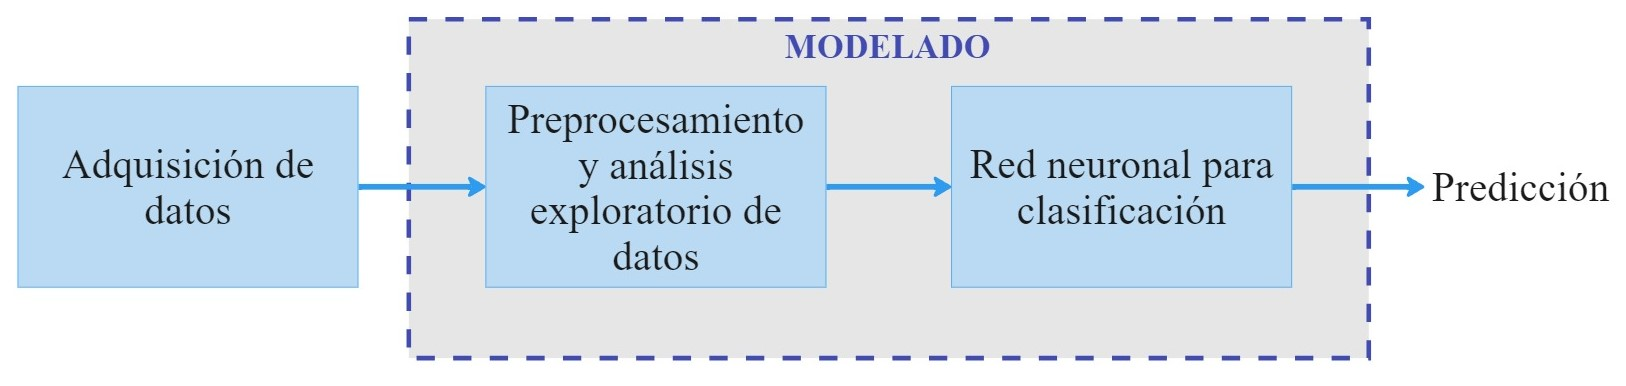
\includegraphics[width=\textwidth]{./Figures/Etapas de trabajo.jpg}
	\caption{Representación esquemática de las etapas del trabajo.}\label{fig:Etapas de trabajo}
\end{figure}

Para comenzar, se llevó a cabo la adquisición de datos. 
Esta etapa fue realizada en colaboración con el servicio de cardiología del Hospital Alemán. 
Para ello, se recopiló información proveniente de presurometrías realizadas a pacientes 
hipertensos a partir del año 2013. Además, se efectuó un análisis exhaustivo de la historia 
clínica de cada paciente con el objetivo de identificar la ocurrencia de eventos cardiovasculares 
adversos mayores. De esta manera, se logró completar el \textit{dataset} con la variable a predecir (MACE) 
para cada paciente. Asimismo, se enriqueció el conjunto de datos con información clínica adicional 
con el fin de contar con variables explicativas más amplias para abordar el problema de investigación.

A continuación, se efectuó una etapa de preprocesamiento. En primer lugar, se procedió a realizar 
una limpieza de los datos con el propósito de seleccionar las variables más representativas del 
problema. Este proceso de selección permitió eliminar datos redundantes, ruidosos o de poca 
utilidad para el análisis posterior. También, se realizó un análisis exploratorio de datos 
para comprender de manera más profunda las características y patrones presentes en el \textit{dataset}. 
Esto proporcionó una visión más completa y significativa del conjunto de datos, permitiendo 
así una mejor comprensión de la naturaleza del problema y orientando la toma de decisiones 
posteriores en el desarrollo de este trabajo.

Por último, se procedió al diseñó y entrenamiento de dos modelos de clasificación utilizando 
redes neuronales. El primer modelo se construyó exclusivamente con los datos de presurometrías, 
mientras que el segundo también incluyó los datos clínicos. El propósito 
de esta estrategia fue analizar y comparar el rendimiento de los dos modelos y evaluar si los 
datos de MAPA tienen un sustento suficiente para predecir la variable objetivo MACE. De esta 
manera, se buscó determinar si la inclusión de información clínica adicional contribuyó a 
mejorar las métricas de desempeño, y si podría tener implicancias 
clínicas relevantes para el seguimiento de los pacientes.

%----------------------------------------------------------------------------------------
%	2.2 ALGORITMOS DE CLASIFICACION
%----------------------------------------------------------------------------------------
\section{Algoritmos de clasificación}
\label{sec:Algoritmos de clasificación}

En esta sección se presentan los fundamentos de los modelos de clasificación, junto con las 
estrategias utilizadas para abordar el desbalance de clases, con especial énfasis en la técnica SMOTE. 
Además, se exploran las métricas utilizadas para evaluar el desempeño de los modelos desarrollados.

%----------------------------------------------------------------------------------------
% 2.2.1 Fundamentos de los modelos de clasificación

\subsection{Fundamentos de los modelos de clasificación}
Un algoritmo de aprendizaje automático es una herramienta que permite resolver tareas  
que suelen ser complejas de abordar para los seres humanos. La principal ventaja del \emph{machine 
learning} (ML) es su capacidad de aprender de los datos y extraer información relevante de 
estos. Las tareas de ML se describen en términos de cómo deben procesar un ejemplo, que se 
compone de una colección de características cuantitativas o \emph{features} que se miden de un objeto 
o evento que se desea procesar. En general, se representa un ejemplo como un vector $ x\in\mathbb{R}^n $,
donde cada entrada $x_{i}$ del vector corresponde a una característica del objeto 
o evento en cuestión. De esta manera, el algoritmo de aprendizaje de máquina es capaz de 
analizar los datos y extraer patrones que permiten tomar decisiones o realizar predicciones 
precisas \citep{CITE:35}.

En el campo del aprendizaje automático, los modelos de clasificación desempeñan un papel fundamental 
\citep{CITE:32}. Estos modelos se encargan de asignar etiquetas discretas o categorías a ejemplos 
específicos según sus características \citep{CITE:33}. Dependiendo del enfoque utilizado durante el 
entrenamiento, los modelos pueden ser de dos tipos: supervisados o no supervisados \citep{CITE:35}.

En un modelo de clasificación no supervisado, las etiquetas no se proporcionan en el conjunto de 
datos de entrenamiento \citep{CITE:34}. En lugar de ello, el algoritmo busca patrones y estructuras 
en los datos sin la guía explícita de las etiquetas. Como resultado, el objetivo es agrupar las instancias en 
clases basadas en similitudes \citep{CITE:33}.

Por otro lado, en un modelo de clasificación supervisado se proporciona al algoritmo un \emph{dataset} de 
entrenamiento que incluye tanto las características de las instancias como las etiquetas correspondientes 
\citep{CITE:33}. El modelo utiliza esta información para aprender a asociar las \emph{features} con las 
etiquetas, lo que le permite clasificar nuevas instancias de manera precisa. Algunos ejemplos de algoritmos 
supervisados ampliamente utilizados son los árboles de decisión, las máquinas de vectores de soporte y 
las redes neuronales \citep{CITE:34}. En este trabajo en particular, se empleó un modelo de clasificación 
supervisado basado en redes neuronales con el propósito de predecir MACE. Es importante señalar que se trata
de una clasificación binaria puesto que la variable \emph{target} tiene dos posibles valores: ausencia ("0") o 
presencia ("1") de eventos cardiovasculares adversos mayores.

%----------------------------------------------------------------------------------------
% 2.2.2 Estrategias para tratar el desbalance de clases
\subsection{Estrategias para tratar el desbalance de clases}

Un conjunto de datos se considera desbalanceado cuando presenta una proporción significativamente mayor 
de observaciones pertenecientes a una clase en comparación con la otra. Este desequilibrio puede tener 
un impacto considerable en el rendimiento de los modelos de aprendizaje automático. En el caso específico 
de una red neuronal entrenada con un \emph{dataset} desbalanceado, es probable que encuentre dificultades 
para discriminar de manera adecuada entre las diferentes clases. En otras palabras, el desequilibrio de 
clases crea un sesgo en el cual el modelo tiende a predecir la clase mayoritaria, lo que dificulta la 
correcta clasificación de los ejemplos pertenecientes a la clase minoritaria \citep{CITE:36} \citep{CITE:37}. 

Abordar el desequilibrio se convierte en un desafío crucial en la tarea de modelado y actualmente existen 
dos enfoques principales. El primero consiste en asignar diferentes pesos a los ejemplos de entrenamiento, 
mientras que el segundo implica realizar un remuestreo del conjunto de datos original. Es posible crear 
un nuevo muestreo del \emph{dataset} efectuando un sobremuestreo de la clase minoritaria y/o un submuestreo 
de la clase mayoritaria. El submuestreo implica una reducción del número de instancias de la clase mayoritaria, 
lo cual puede resultar en la pérdida de información valiosa que sea representativa de la distribución de los 
datos. Por otra parte, el sobremuestreo suele incluir réplicas de ejemplos de la clase minoritaria, lo cual 
puede generar un sobreajuste. Cabe señalar que un modelo sobreajustado concede predicciones 
muy precisas para el conjunto de entrenamiento pero no logra generalizar adecuadamente cuando se presentan 
nuevos datos \citep{CITE:37}. 

Para mitigar las desventajas mencionadas anteriormente, Nitesh Chawla \emph{et al.} \citep{CITE:37} 
introducen una nueva técnica que implica una forma especial 
de sobremuestrear la clase minoritaria. El algoritmo 
\emph{Synthetic Minority Over-sampling Technique} (SMOTE) implica la creación de muestras sintéticas de 
la clase minoritaria. Se expone una representación gráfica del algoritmo en la figura \ref{fig:SMOTE}. 
En primer lugar, el método escoge un ejemplo de la clase minoritaria al azar y encuentra a sus $k$ vecinos 
más cercanos. Luego, se selecciona uno de los $k$ vecinos más cercanos y se crea una conexión mediante 
un segmento de línea en el espacio de características con la muestra elegida al azar. Finalmente, se crea 
una instancia sintética en un punto aleatorio entre los dos ejemplos. Este procedimiento se repite para
todas las muestras minoritarias \citep{CITE:38}. 

\begin{figure}[h!]
	\centering
	\subcaptionbox{SMOTE comienza con un conjunto de ejemplos positivos (puntos verdes) y negativos (puntos azules).}%
  	[0.3\linewidth]{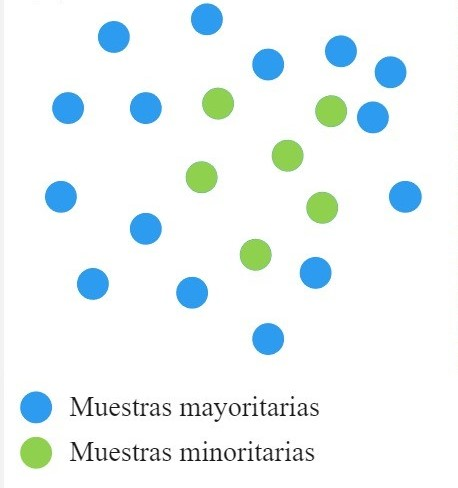
\includegraphics[height=5cm]{./Figures/SMOTE_a.jpg}}\label{fig:SMOTEa}
	\hspace{1em}
	\subcaptionbox{Se selecciona un ejemplo positivo (punto con borde negro) y sus $k$ vecinos más cercanos entre los positivos (puntos amarillos, con $k = 3$).}
	[0.3\linewidth]{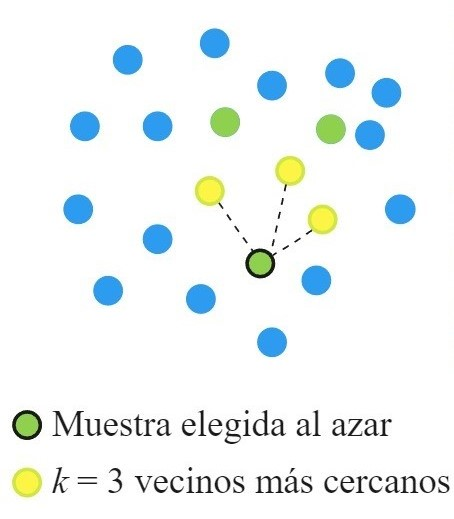
\includegraphics[height=5cm]{./Figures/SMOTE_b.jpg}}\label{fig:SMOTEb}
	\hspace{1em}
	\subcaptionbox{Para cada $k$ vecino más cercano se agrega un nuevo ejemplo sintético (puntos rojos) a lo largo de la línea recta que los conecta con el ejemplo positivo.}
	[0.3\linewidth]{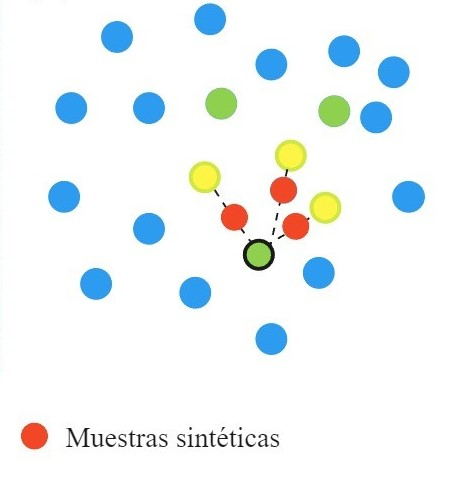
\includegraphics[height=5cm]{./Figures/SMOTE_c.jpg}}
	\caption{Representación esquematica del algoritmo SMOTE\protect\footnotemark.}\label{fig:SMOTEc}
	   \label{fig:SMOTE}
\end{figure}


En suma, SMOTE permite generar ejemplos sintéticos que sean relativamente cercanos en el espacio de 
características con respecto a las muestras existentes de la clase minoritaria. Además, las muestras 
pueden crearse en la cantidad que sea requerida. Por lo tanto, en escenarios donde el conjunto de 
datos no solo está desbalanceado sino que también presenta una escasez de muestras, la aplicación 
de SMOTE resulta particularmente efectiva \citep{CITE:37} \citep{CITE:38}.


%----------------------------------------------------------------------------------------
% 2.2.3 Métricas de evaluación en modelos de clasificación
\subsection{Evaluación de modelos de clasificación}

% el footnote text es de la imagen de smote, pero si lo ponia mas arriba lo corria en la pagina anterior
\footnotetext{Imagen adaptada de Schubach, Max; Re, Matteo; Robinson, Peter y Valentini, Giorgio. (2017). Imbalance-Aware Machine Learning for Predicting Rare and Common Disease-Associated Non-Coding Variants. Scientific Reports. 7. 10.1038/s41598-017-03011-5.}

Para evaluar el desempeño de un modelo de clasificación binaria se suele emplear una matriz de confusión. 
Esta matriz se ilustra en la figura \ref{fig:MatrizConfusion}, donde las columnas representan la clase 
predicha y las filas corresponden a las clases reales \citep{CITE:44}. 
A partir de esta tabla, se definen cuatro indicadores:

\begin{itemize}
	\item Verdaderos positivos (TP, por sus siglas en inglés): asignaciones positivas correctas.
	\item Verdaderos negativos (TN, por sus siglas en inglés): asignaciones negativas correctas.
\item Falsos positivos (FP, por sus siglas en inglés): asignaciones positivas incorrectas, es decir que
indican la presencia de una condición cuando la misma en realidad no está presente.
\item Falsos negativos (FN, por sus siglas en inglés): asignaciones negativas incorrectas, lo que significa
que indican la ausencia de una condición cuando en realidad está presente.
\end{itemize}

\begin{figure}[h!]
	\centering
	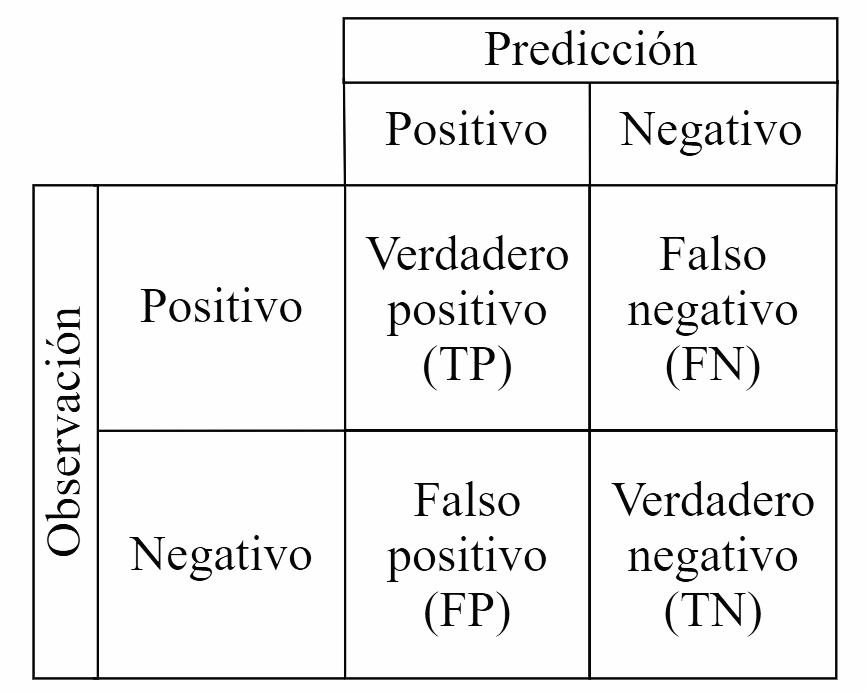
\includegraphics[width=0.5\textwidth]{./Figures/MatrizConfusion.jpg}
	\caption{Matriz de confusión\protect\footnotemark.}\label{fig:MatrizConfusion}
\end{figure}


En el ámbito médico, el falso negativo puede ocasionar las consecuencias más graves para la salud del 
paciente. En este trabajo en particular, implica el riesgo de no tomar las medidas necesarias para un 
tratamiento adecuado, lo cual puede incurrir en que el paciente experimente un evento cardiovascular 
adverso mayor. En consecuencia, es de gran importancia minimizar la tasa de falsos negativos al máximo, 
aún si esto implica un aumento de falsos positivos. Si bien este incremento puede implicar la necesidad de 
destinar más recursos médicos para realizar pruebas adicionales o tratamientos innecesarios, se garantiza 
que menos casos sean pasados por alto \citep{CITE:40}.

\filbreak

% el footnote text es de la imagen de MatrizConfusion, pero si lo ponia mas arriba lo corria en la pagina anterior
\footnotetext{Imagen adaptada de Portilla, Jose. 2018. Data Science and Machine Learning Bootcamp with R. https://www.udemy.com/data-science-and-machine-learning-bootcamp-with-r/.}

A partir de los valores de TP, TN, FP y FN se definen diferentes métricas para evaluar el desempeño de 
un modelo de clasificación. A continuación, se explican algunas en detalle.

\subsubsection{\emph{Precision}}
La presición o \emph{precision} es una métrica que permite conocer la proporción de ejemplos clasificados 
correctamente como positivos sobre el total de ejemplos clasificados como positivos. Una alta precisión 
indica que el modelo tiene una baja tasa de falsos positivos y clasifica correctamente la mayoría de las 
instancias positivas. La expresión matemática que describe este comportamiento es la siguiente:

\begin{equation}
	\label{eq:precision}
	Precision = \frac{TP}{TP + FP}
\end{equation}


\subsubsection{\emph{Recall}}
La sensibilidad, \emph{recall} o tasa positiva real (TPR) es una métrica que mide la proporción de ejemplos 
clasificados correctamente como positivos en relación con el total de ejemplos positivos. Por lo tanto, se 
mide la capacidad de identificar la mayoría de las muestras positivas presentes. La ecuación que describe 
a la sensibilidad es:

\begin{equation}
	\label{eq:recall}
	Recall = \frac{TP}{TP + FN}
\end{equation}


\subsubsection{\emph{F1 score}}
La métrica \emph{F1 score} es la media armónica entre \emph{precision} y \emph{recall}. Dado que tiene 
en cuenta tanto a los FP cómo los FN, se emplea para evaluar un modelo cuando el conjunto de datos es 
desequilibrado. La fórmula matemática que describe este comportamiento es la siguiente:

\begin{equation}
	\label{eq:f1score}
	F1\,score = \frac{2}{\nicefrac{1}{Precision} + \nicefrac{1}{Recall}} = 2\cdot\frac{Recall \cdot Precision}{Recall + Precision}
\end{equation}

\subsubsection{\emph{Accuracy}}
La exactitud o \emph{accuracy} es una métrica que mide la proporción de muestras clasificadas correctamente 
sobre el total de muestras evaluadas y se describe matemáticamente como:

\begin{equation}
	\label{eq:accuracy}
	Accuracy = \frac{TP + TN}{TP + TN + FP + FN}
\end{equation}

\subsubsection{\emph{Specificity}}
La especificidad, \emph{specificity} o tasa negativa real (TNR) se define como la proporción de falsos positivos 
sobre el total de negativos reales. Es una métrica exactamente opuesta a la sensibilidad y esta dada por:

\begin{equation}
	\label{eq:specificity}
	Specificity = \frac{TN}{TN + FP}
\end{equation}


\subsubsection{Curva ROC y AUC}
La curva ROC es una representación gráfica que muestra la tasa de verdaderos positivos (sensibilidad)
en función de la tasa de falsos positivos (1 - especificidad) a medida que se varía el umbral de 
clasificación. Si bien puede ser de utilidad visualizar la curva ROC, en muchas casos la información 
puede resumirse en la métrica AUC (acrónimo de \emph{Area Under the Curve}), que mide el área bajo la curva 
ROC. En general, cuanto más alto sea el AUC, mejor es el desempeño del clasificador \citep{CITE:37} \citep{CITE:44}. 

En la figura \ref{fig:ROC_a}, se puede observar un clasificador ideal en el cual las curvas de TP y TN no se 
superponen en absoluto, lo que resulta en un AUC igual a 1. Por el contrario, en la figura \ref{fig:ROC_c}, 
se muestra un clasificador de predicción aleatoria, donde la curva ROC es una línea recta con una pendiente unitaria. 
En este caso, las curvas de TP y TN se superponen por completo, lo que da como resultado un AUC de 0.5. 
En la figura \ref{fig:ROC_b}, se observa un caso intermedio en el que hay cierta superposición entre las curvas 
de TP y TN. En general, la mayoría de los modelos de clasificación binaria tienen un AUC entre 0.5 y 1. Es poco 
común encontrar un clasificador con un AUC menor que 0.5, ya que esto indicaría que las predicciones están invertidas \citep{CITE:44}.

\begin{figure}[h!]
	\centering
	\subcaptionbox{Clasificador perfecto.\label{fig:ROC_a}}%
  	[0.3\linewidth]{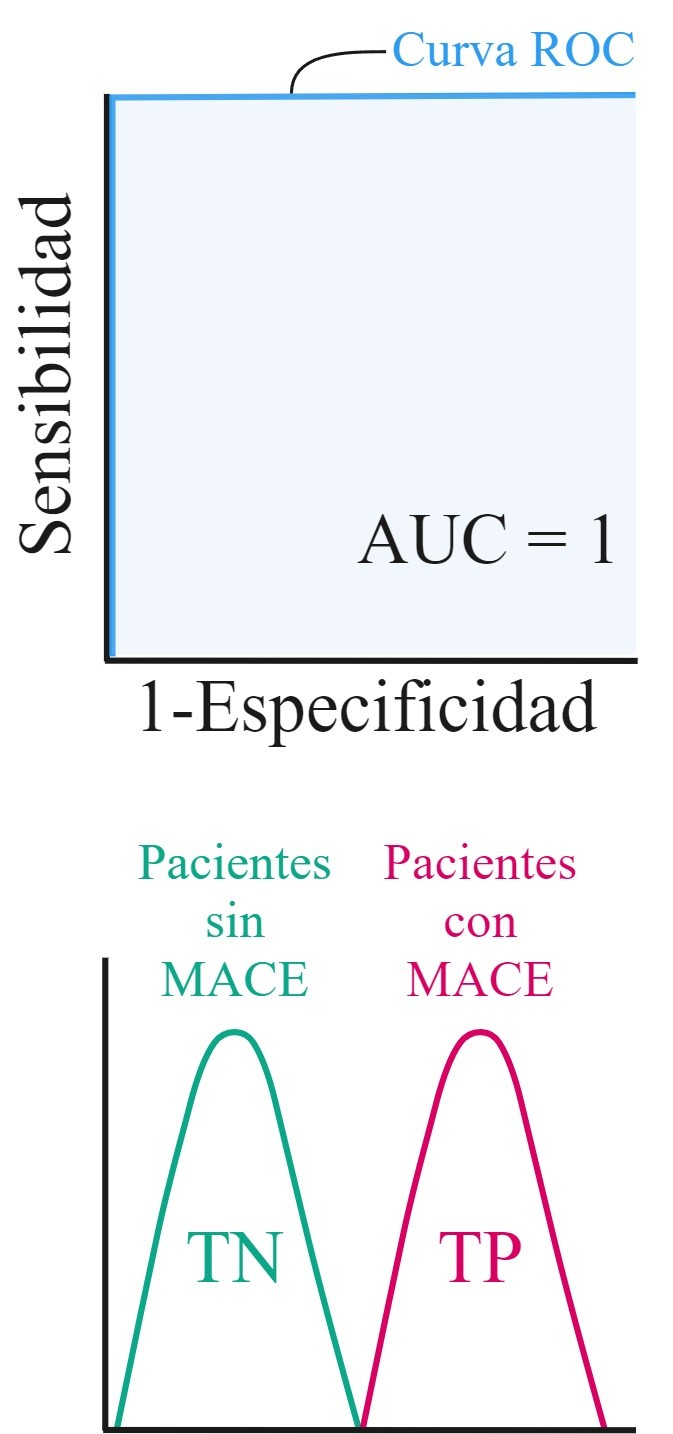
\includegraphics[height=8cm]{./Figures/ROC_a.jpg}}
	\hspace{1em}
	\subcaptionbox{Clasificador con buen \\poder predictivo.\label{fig:ROC_b}}
	[0.3\linewidth]{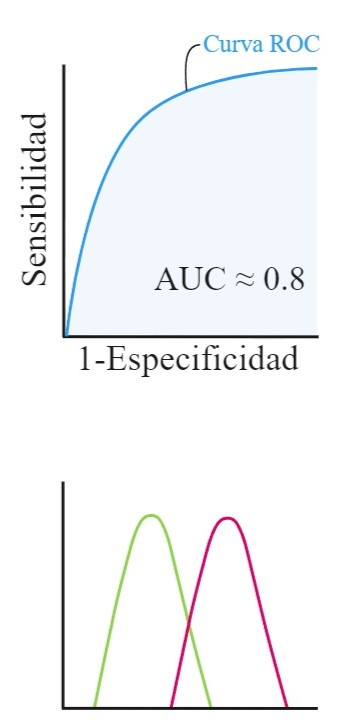
\includegraphics[height=8cm]{./Figures/ROC_b.jpg}}
	\hspace{1em}
	\subcaptionbox{Clasificador sin poder predictivo.\label{fig:ROC_c}}
	[0.3\linewidth]{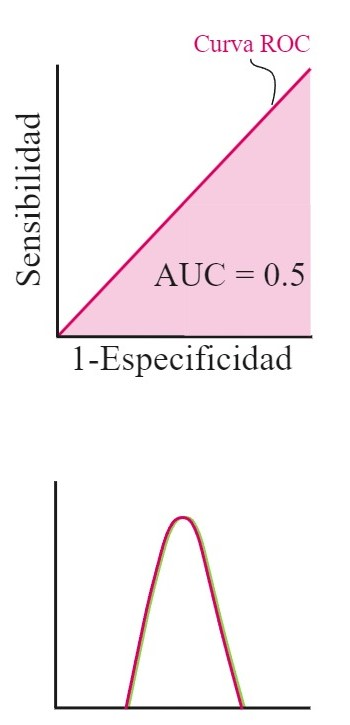
\includegraphics[height=8cm]{./Figures/ROC_c.jpg}}
	\caption{Representación gráfica de la curva ROC y las distribuciones de TP y TN\protect\footnotemark.}
\end{figure}

Para el presente trabajo, se evaluaron todas las métricas mencionadas anteriormente. Sin embargo, se seleccionó 
el AUC como la métrica principal para medir el desempeño de los modelos. Esto se debe a que en el ámbito clínico 
resulta de gran relevancia analizar la relación de compromiso entre la sensibilidad y especificidad. En definitiva, 
se buscó encontrar un equilibrio óptimo entre la detección temprana de casos de MACE positivos (alta sensibilidad) 
y la minimización de falsas alarmas (alta especificidad). 


%----------------------------------------------------------------------------------------
%	2.3 PERCEPTRÓN MULTICAPA
%----------------------------------------------------------------------------------------
\filbreak
\section{Perceptrón multicapa}
\label{sec:Perceptrón multicapa}

% el footnote text es de la imagen de ROC, pero si lo ponia mas arriba lo corria en la pagina anterior
\footnotetext{Imagen adaptada de Glen, S. (2019). ROC Curve Explained in One Picture. Data Science Central. https://www.datasciencecentral.com/roc-curve-explained-in-one-picture/.}

Las redes neuronales artificiales (RNA), propuestas inicialmente por McCulloch y Pitts en 1943 
\citep{CITE:41}, son modelos computacionales que se inspiran en el funcionamiento del cerebro 
humano. Si bien existen diversos tipos de RNA, esta sección se centra en los perceptrones 
multicapa, puesto que es la red empleada en este trabajo. En particular, se abordan varios 
aspectos teóricos clave relacionados con los perceptrones multicapa, incluyendo los bloques 
fundamentales que componen esta red, el algoritmo de entrenamiento, la validación del modelo, 
los hiperparámetros y los optimizadores.

%----------------------------------------------------------------------------------------
% 2.3.1 Perceptrón
\subsection{Perceptrón}
Un perceptrón, también conocido como neurona artificial o nodo, es el bloque fundamental de las 
RNA y fue propuesto por Frank Rosenblatt en 1957 \citep{CITE:43}. En la figura \ref{fig:Perceptron} se puede observar 
cómo un perceptrón recibe $n$ señales de entrada $x = (x_1, x_2, …, x_n)$, las cuales se multiplican 
por un peso $W = (w_1, w_2, …, w_n)$. Este comportamiento es análogo a la manera en que los 
pesos sinápticos influyen en las neuronas biológicas, ya que algunas entradas tienen mayor relevancia 
que otras. Por este motivo, las entradas se combinan como una suma ponderada por sus pesos 
($\sum_{i=1}^{n} W_i^T \cdot x_i$) y se añade un término independiente conocido como \emph{bias} o 
sesgo, con el fin de otorgar flexibilidad en la modelización de patrones complejos. 
Posteriormente, se aplica una transformación no lineal mediante una función de activación $g$, 
la cual determina la salida $\hat{y}$ del perceptrón \citep{CITE:35} \citep{CITE:42}. 
La descripción matemática de este comportamiento se expresa de la siguiente manera: 

\begin{equation}\label{eq:perceptron}
\begin{split}
	&\hat{y} = g(z) = g( \sum_{i=1}^{n} W^T \cdot x + b) \\
				&\hat{y} = g(x_1 \cdot w_1 + x_1 \cdot w_1 + … + x_n \cdot w_n + b)
\end{split}
\end{equation}

\begin{figure}[h!]
	\centering
	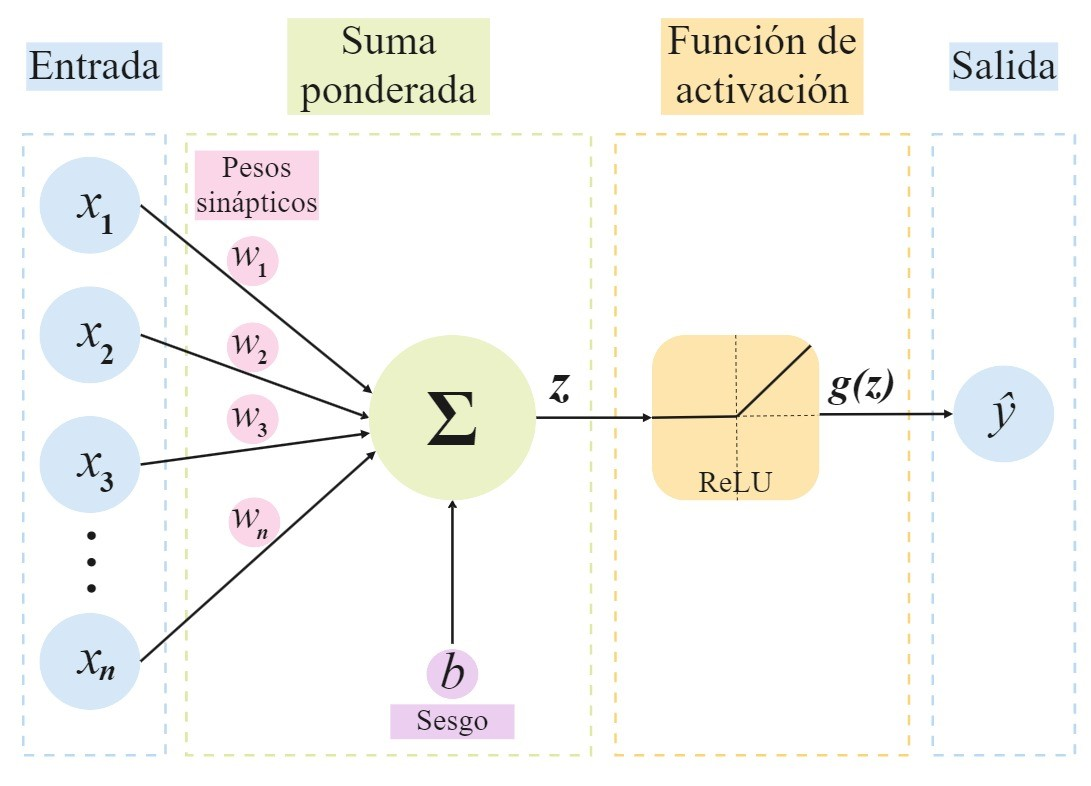
\includegraphics[width=\textwidth]{./Figures/Perceptron.jpg}
	\caption{Representación de un perceptrón\protect\footnotemark.}
	\label{fig:Perceptron}
\end{figure}


\footnotetext{Imagen adaptada de Hange, A. (2021). Target Prediction using Single-layer Perceptron and Multilayer Perceptron. Nerd For Tech. https://medium.com/nerd-for-tech/flux-prediction-using-single-layer-perceptron-and-multilayer-perceptron-cf82c1341c33/.}

%----------------------------------------------------------------------------------------
% 2.3.2 Arquitectura del perceptrón multicapa
\subsection{Arquitectura del perceptrón multicapa}

Un perceptrón multicapa (MLP, por sus siglas en inglés), también conocido como \emph{feedforward neural network} es 
una arquitectura de RNA ampliamente utilizada en el campo del aprendizaje profundo. Como se aprecia en la figura \ref{fig:MLP}, 
un MLP está compuesto por tres capas: capa de entrada o \emph{input layer}, capa oculta 
o \emph{hidden layer} y capa de salida o \emph{output layer}. 
A su vez, cada capa está formada por neuronas artificiales. La arquitectura del MLP es conocida como \emph{feedforward} 
puesto que la información siempre fluye desde la capa de entrada hacia la capa de salida a través de las capas ocultas, 
sin conexiones de retroalimentación. Cuando una RNA tiene dos o más capas ocultas, se lo conoce como una red neuronal 
profunda o \emph{deep neural network} (DNN) \citep{CITE:35} \citep{CITE:44}. 

\begin{figure}[h!]
	\centering
	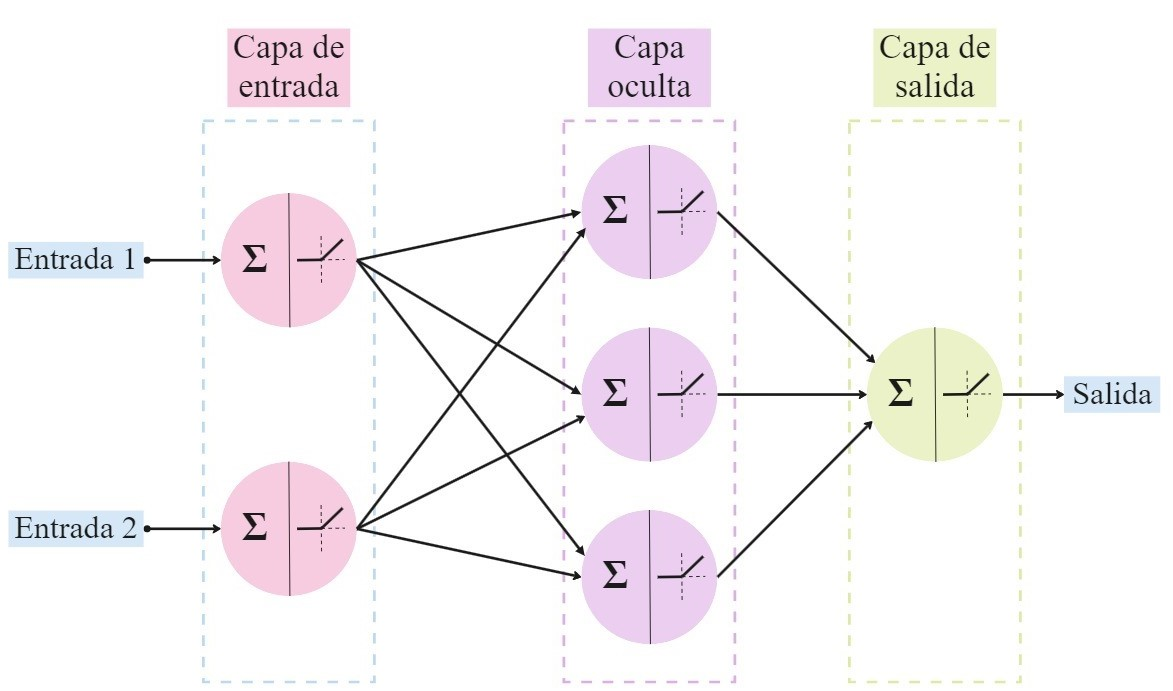
\includegraphics[width=\textwidth]{./Figures/MLP.jpg}
	\caption{Representación de un perceptrón multicapa \\ \emph{fully connected}\protect\footnotemark.}
	\label{fig:MLP}
\end{figure}

Por otro lado, el número de neuronas en la capa de entrada está definido por la cantidad de variables independientes 
del modelo, mientras que el número de nodos de la salida es la cantidad de variables dependientes. Además, el número de 
capas ocultas y su cantidad de neuronas dependen de la complejidad del modelo en cuestión, y son parámetros importantes 
a tener en cuenta durante el desarrollo de la red\citep{CITE:42}.

La configuración del perceptrón multicapa de la figura \ref{fig:MLP} se conoce como \emph{fully connected}, ya que todos 
los nodos de una capa están conectados con todos los nodos de las capas adyacentes. Sin embargo, existen otros tipos de 
capas que poseen diferentes estructuras de conexión. Por ejemplo, las de abandono o \emph{dropout} introducen la omisión de 
algunos nodos durante el entrenamiento de forma aleatoria para reducir el sobreajuste \citep{CITE:44} \citep{CITE:45}.

En general, la función de activación comúnmente empleada en las capas ocultas es la unidad lineal rectificada (ReLU, 
por sus siglas en inglés). La elección de ReLU se basa en dos ventajas principales: su implementación es rápida y no 
tiene un valor máximo de salida. En consecuencia, se evitan ciertos problemas durante el descenso del gradiente. En la 
ecuación \ref{eq:relu}, se observa que si el valor de entrada $z$ es negativo, la función retorna un 0; de lo contrario, 
devuelve el valor de $z$ \citep{CITE:44}. 

\footnotetext{Imagen adaptada de Hange, A. (2021). Target Prediction using Single-layer Perceptron and Multilayer Perceptron. Nerd For Tech. https://medium.com/nerd-for-tech/flux-prediction-using-single-layer-perceptron-and-multilayer-perceptron-cf82c1341c33/.}

\begin{equation}
	\label{eq:relu}
	ReLU(z) = max(0, z)
\end{equation}

Por otro lado, en la capa de salida de un modelo de clasificación binaria, es común utilizar la función sigmoide o 
\emph{sigmoid}. Esta función, definida en la ecuación \ref{eq:sigmoid}, toma valores reales como entrada y genera 
valores de salida en el rango de 0 a 1. Así, la función sigmoide es útil para predecir la probabilidad de una 
variable binaria \citep{CITE:44}. 

\begin{equation}
	\label{eq:sigmoid}
	\sigma(z) = \frac{1} {1 + e^{-z}}
\end{equation}


%----------------------------------------------------------------------------------------
% 2.3.3 Algoritmo de entrenamiento
\subsection{Algoritmo de entrenamiento}
El perceptrón multicapa se entrena con el fin de minimizar el error entre la salida deseada $y$ y 
la salida computada por el modelo $\hat{y}$ empleando una función de pérdida o \emph{loss function}. 
En el caso de problemas de clasificación binaria, se utiliza una función llamada 
\emph{binary cross entropy} (BCE), que se define como:

\begin{equation}
	\label{eq:BCE}
	\mathcal{L} = -\frac{1}{N} \sum_{i=1}^Ny_{i}\cdot\log(\hat{y_{i}}) + (1 - y_{i})\cdot\log(1 - \hat{y_{i}})
\end{equation}

Como resultado, cuando la salida verdadera es $y_{i} = 1$, la probabilidad de clasificarlo como 
1 es  $\hat{y_{i}}$, lo que hace que el segundo término se anule. Por el contrario, cuando la 
salida verdadera es $y_{i} = 0$, la probabilidad de clasificarlo como 1 es  $1 - \hat{y_{i}}$, 
lo que hace que se cancele el primer término. De esta forma, al aplicar el logaritmo, la BCE 
penaliza en mayor medida cuando el modelo clasifica incorrectamente con alta confianza \citep{CITE:46}. 
En consecuencia, si la red produce una respuesta equivocada, los pesos se actualizan para minimizar el error. 
Esto conduce a una reducción de los errores y aumenta la probabilidad de que las salidas futuras de la red 
sean correctas. En la práctica, el algoritmo de aprendizaje de un MLP involucra una etapa de propagación 
hacia adelante (\emph{forward propagation}) seguida de una etapa de propagación hacia atrás (\emph{backward propagation} 
o \emph{backpropagation}) \citep{CITE:35}. A continuación, se describen brevemente estas etapas.

\subsubsection{Propagación hacia adelante}
La fase de propagación hacia adelante implica el flujo de información desde la capa de entrada hacia la de 
salida de la red neuronal, con el objetivo de realizar una predicción. La salida de la n-ésima capa se 
define en la ecuación \ref{eq:forward}, donde $h^{(n)}$ es la salida, $g^{(n)}$ es la función de activación, $W^{(n)}$ 
es la matriz de pesos y $b^{(n)}$ es el vector de sesgos \citep{CITE:35} \citep{CITE:44}.

\begin{equation}
	\label{eq:forward}
	h^{(n)} = g^{(n)} (W^{(n)T} \cdot h^{(n-1)} + b^{(n)})
\end{equation}

El algoritmo~\ref{alg:forward} describe el proceso de \emph{forward propagation} en una red neuronal de profundidad $n$. 
Luego de calcular la predicción $\hat{y}$, se calcula la función de costo total $J$ durante la fase de entrenamiento. 
Esta se define como la suma de la función de pérdida $\mathcal{L}$ y un término de regularización $\lambda \Omega(w)$.

\floatname{algorithm}{Algoritmo}
\begin{algorithm}
	\caption{Propagación hacia adelante de una RNA con $n$ capas.}
	\label{alg:forward}
	\begin{algorithmic}
		\Require $W^{(i)}, i \in 1, \ldots, n$ 
		\Require $b^{(i)}, i \in 1, \ldots, n$ 
		\Require $x$ 
		\Require $y$ 
		\State $h^{(1)} \gets x$
		\For{$m \gets 1, \ldots, n$}
		\State $a^{(m)} \gets W^{(m)T}h^{(m-1)} + b^{(m)} $
		\State $h^{(m)} \gets g(a^{(m)})$
		\EndFor
		\State $\hat{y} \gets h^{(n)}$
		\State $J \gets \mathcal{L}(\hat{y}, y) + \lambda \Omega(w)$ \Comment{\small Si es fase de entrenamiento.}
	\end{algorithmic}
\end{algorithm}

\subsubsection{Retropropagación}

Durante muchos años, los investigadores se enfrentaron al desafío de encontrar una forma 
efectiva de entrenar a los perceptrones multicapa sin éxito. Sin embargo, en 1986, D. E. 
Rumelhart \emph{et al.} publicaron un artículo revolucionario que introdujo el método 
de \emph{backpropagation} \citep{CITE:47}. La fase de retropropagación se describe en el 
algoritmo~\ref{alg:backpropagation}. Esta implica el cálculo del gradiente de la función de 
costo respecto a todos los parámetros entrenables empleando la regla de la cadena. 
Luego, este gradiente se propaga desde la salida hacia la entrada de la red neuronal \citep{CITE:35} \citep{CITE:42} \citep{CITE:44}.

\begin{algorithm}[H]
	\caption{Propagación hacia atrás de una RNA con $n$ capas.}
	\label{alg:backpropagation}
		\begin{algorithmic}
		\State $g \gets \nabla_{\hat{y}} J = \nabla_{\hat{y}} \mathcal{L}(\hat{y}, y)$ \Comment{\small Cálculo del gradiente en la capa de salida.}
		\For{$m \gets n, n-1, \ldots, 1$}
		\State $g \gets \nabla_{a^{(m)}} J = g \odot f'(a^{(m)})$ \Comment{Actualiza el gradiente $g$.}
		\State $\nabla_{b^{(m)}} J = g + \lambda \nabla_{b^{(m)}} \Omega(w)$ \Comment{\small Cálculo del gradiente respecto a $b^{(m)}$.}
		\State $\nabla_{W^{(m)}} J = g h^{(m-1)} + \lambda \nabla_{W^{(m)}} \Omega(w)$ \Comment{\small Cálculo del gradiente respecto a $W^{(m)}$.}
		\State $g \gets \nabla_{h^{(m-1)}} J = W^{(m)T}g$ \Comment{\small Propagación del gradiente.}
		\EndFor
	\end{algorithmic}
\end{algorithm}
%----------------------------------------------------------------------------------------
% 2.3.4 Validación del modelo
\subsection{Validación del modelo}
Para el desarrollo de una RNA, es necesario dividir al conjunto de datos en dos subconjuntos: uno para el 
entrenamiento y otro para la validación o prueba. El conjunto de entrenamiento se emplea para entrenar a 
la red, mientras que el conjunto de prueba se utiliza para evaluar su desempeño. Es crucial asegurarse de 
que el conjunto de entrenamiento sea lo suficientemente grande y representativo del problema, mientras 
que el de prueba sea lo suficientemente grande para facilitar una correcta validación de la red. En casos 
donde el número de ejemplos disponible no es suficiente para realizar la división representativa, se 
pueden utilizar otras estrategias \citep{CITE:42}. 
El procedimiento mayormente empleado es la validación cruzada de $k$ 
iteraciones, también conocida como \emph{k-fold cross validation}, que se ilustra en la figura \ref{fig:crossval}. 

\begin{figure}[h!]
	\centering
	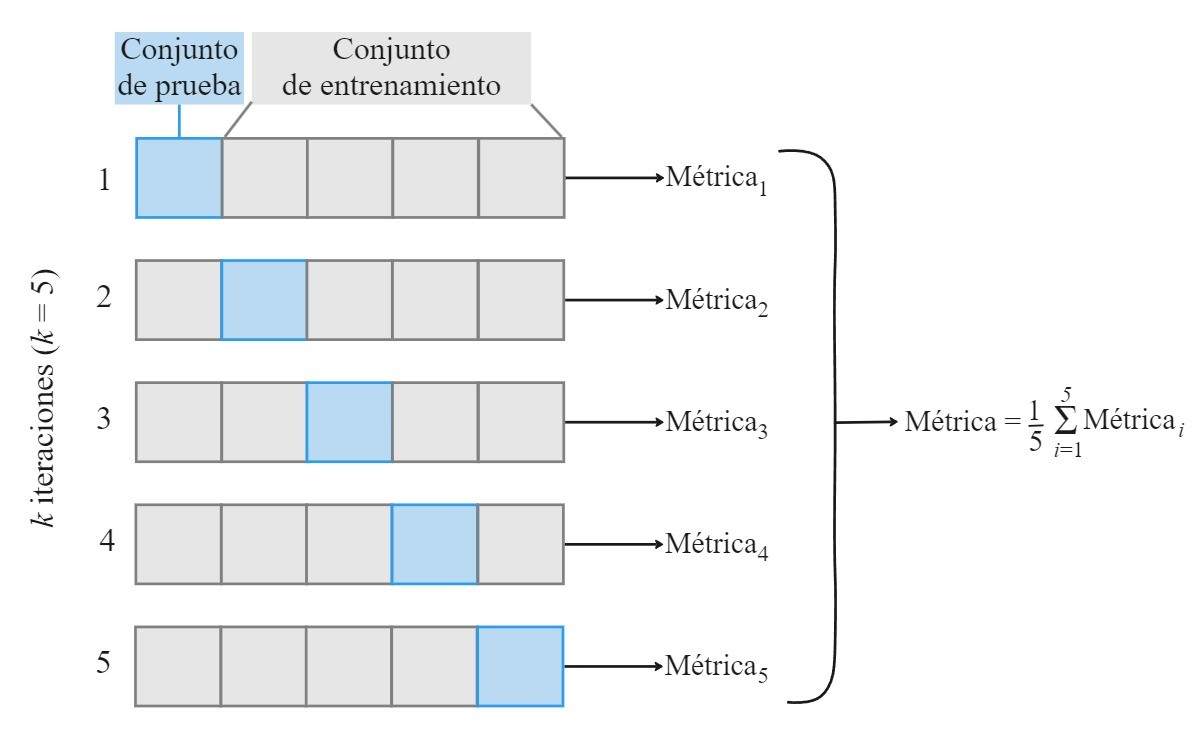
\includegraphics[width=\textwidth]{./Figures/cross_validation.jpg}
	\caption{Representación esquemática de \emph{k-fold cross validation} con $k=5$\protect\footnotemark.}
	\label{fig:crossval}
\end{figure}


La validación cruzada de $k$ iteraciones consiste en dividir el conjunto de datos en $k$ subconjuntos. Durante 
el proceso de entrenamiento, se toma cada $k$ subconjunto como el conjunto de prueba, mientras que los 
restantes ($k-1$) se utilizan como conjunto de entrenamiento. Este proceso se repetie $k$ veces, donde 
en cada iteración se toma un conjunto de prueba diferente y los datos remanentes forman el conjunto 
de entrenamiento. Al finalizar las $k$ iteraciones, se calcula el promedio de las métricas y error 
obtenidos para cada subconjunto de prueba \citep{CITE:48}.

%----------------------------------------------------------------------------------------
% 2.3.5 Optimización del modelo
\filbreak
\subsection{Optimización del modelo}
Es fundamental comprender el papel de los optimizadores y su impacto en el entrenamiento de una red neuronal. 
Los optimizadores son un algoritmos empleados para ajustar los parámetros de la red, con el fin de minimizar 
la función de pérdida. Como resultado, logran mejorar la capacidad de aprendizaje y rendimiento del modelo. 
Algunos optimizadores comúnmente utilizados incluyen: descenso de gradiente estocástico, AdaGrad, Adam y RMSprop. 
Cada uno de ellos posee sus propias características y métodos de actualización de parámetros. Por lo tanto, 
la elección del optimizador es un paso importante en el desarrollo de un modelo, ya que puede influir 
significativamente en la velocidad y calidad de convergencia durante el entrenamiento \citep{CITE:44}.

\footnotetext{Imagen adaptada de Ashfaque Maat, Johar y Iqbal, Amer. (2019). Introduction to Support Vector Machines and Kernel Methods.}

En particular, el algoritmo de optimización empleado en este trabajo fue propuesto por 
Diederik Kingma y Jimmy Ba en su artículo ``\emph{Adam: A Method for Stochastic Optimization}'' \citep{CITE:49}. Si bien 
la elección del optimizador depende de diversos factores, Adam se destaca por múltiples ventajas, que incluyen:

\begin{itemize}
	\item Implementación sencilla.
	\item Eficiencia computacional.
	\item Requisitos de memoria reducidos.
	\item Invarianza a la reescala diagonal de los gradientes.
	\item Adecuación para problemas con muchos datos y/o parámetros.
	\item Idoneidad para problemas con gradientes muy ruidosos o dispersos.
	\item Hiperparámetros con interpretación intuitiva que generalmente requieren poco ajuste.
\end{itemize}


%----------------------------------------------------------------------------------------
% 2.3.6 Hiperparámetros del modelo
\subsection{Hiperparámetros del modelo}
En los modelos de aprendizaje automático, los parámetros son las variables que se estiman durante el 
proceso de entrenamiento con el conjunto de datos. Por otro lado, los hiperparámetros del modelo 
corresponden a los valores de configuración que se emplean durante dicho proceso. A diferencia de 
los parámetros, los hiperparámetros no son afectados por el algoritmo de aprendizaje. Por lo tanto, 
deben ser establecidos antes del entrenamiento y se mantienen constantes durante el mismo \citep{CITE:44}.

Usualmente, gran parte del diseño de una RNA implica la selección y ajuste de los hiperparámetros. 
Una elección adecuada puede tener un impacto significativo en el desempeño del modelo, ya que estos 
determinan el comportamiento y la capacidad de aprendizaje de la red. Algunos hiperparámetros 
que pueden ser ajustados incluyen: cantidad y tipo de capas ocultas, cantidad de neuronas en cada capa,
función de activación, función de pérdida, optimizador, tasa de aprendizaje, tamaño del lote y
número de épocas de entrenamiento \citep{CITE:35} \citep{CITE:42} \citep{CITE:44}.


 
%\chapter{Diseño e implementación} % Main chapter title

\label{Chapter3} % Change X to a consecutive number; for referencing this chapter elsewhere, use \ref{ChapterX}

En este capítulo, se presentan de manera concisa las decisiones de diseño del sistema. 
Se abordan aspectos clave como la adquisición de datos, las técnicas de preprocesamiento 
utilizadas y el diseño del modelo de aprendizaje profundo. 

%----------------------------------------------------------------------------------------
%	ADQUISICION DE DATOS
%----------------------------------------------------------------------------------------
\section{Adquisición de datos}
 
\newcommand{\myhash}{\raisebox{\depth}{\#}}

Para llevar a cabo el presente trabajo, se emplearon datos proporcionados por el servicio 
de cardiología e hipertensión del Hospital Alemán. La figura \ref{fig:adquisicion_datos} 
exhibe un diagrama en bloques que ilustra la etapa de adquisición de datos utilizada. 
Es importante destacar que se utilizaron dos conjuntos de datos diferentes. 

\begin{figure}[H]
	\centering
	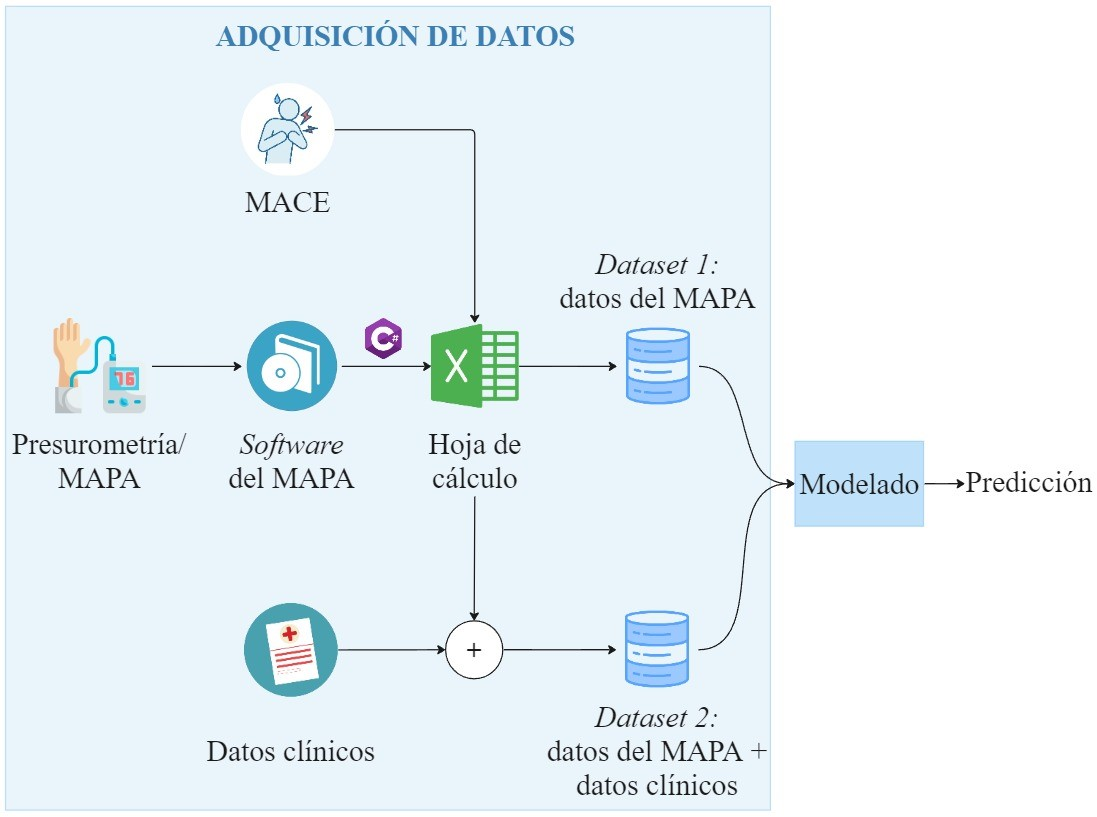
\includegraphics[width=\textwidth]{./Figures/adquisicion_datos2.jpg}
	\caption{Representación esquemática de la etapa de adquisición de datos.}\label{fig:adquisicion_datos}
\end{figure}

El primer \emph{dataset} se compone exclusivamente de información recopilada de las 
presurometrías realizadas a los pacientes hipertensos a partir del año 2013. Luego 
de realizar un MAPA, los datos se almacenan en un \emph{software} especializado de 
los presurómetros. Posteriormente, se extraen utilizando un programa desarrollado 
en C\# para ser registrados en una planilla de cálculo. Sumado a esto, se incluyó 
la variable a predecir (MACE) para cada paciente mediante un análisis exhaustivo 
de su historial clínico. Especificamente, se registró la ocurrencia de 
un accidente cerebrovascular no fatal, infarto agudo de miocardio, insuficiencia 
cardíaca, insuficiencia renal crónica o muerte. En caso de que correspondiera, también 
se incluyó la fecha correspondiente en la que tuvo lugar el evento.

Por otro lado, el segundo conjunto de datos contiene información adicional obtenida 
del historial clínico de cada paciente. Estos datos clínicos se agregan a la misma 
hoja de cálculo mencionada anteriormente, complementando así la información proveniente 
de las presurometrías.

El objetivo de utilizar dos \emph{datasets} es evaluar la calidad de los datos de 
las presurometrías para generar inferencias de manera independiente. En otras palabras, 
se buscó determinar en qué medida los datos del MAPA pueden ser utilizados por sí solos 
para obtener predicciones significativas y precisas de MACE. Al mismo tiempo, se procuró 
evaluar si la incorporación de información clínica contribuye a un mejor desempeño del 
modelo en términos de tasa de falsos negativos, AUC y otras métricas relevantes.


%----------------------------------------------------------------------------------------
% 3.1.1 Descripción del conjunto de datos

\subsection{Descripción del conjunto de datos}

El primer conjunto de datos comprende las variables derivadas del MAPA, junto con 
el valor de MACE y la fecha del evento asociado. A continuación, se brinda una 
descripción detallada de las variables provenientes de las presurometrías: 

\begin{itemize}
  \item Fechaest: corresponde a la fecha en la cual se realizó la presurometría.
  \item PASm24: representa la presión arterial sistólica media durante todo el MAPA.
	\item PADm24: representa la presión arterial diastólica media durante todo el MAPA.
  \item FCm24: representa la frecuencia cardíaca media durante todo el MAPA.
  \item PAMm24: representa la presión arterial media durante todo el MAPA.
  \item PPm24: representa la presión de pulso media durante todo el MAPA.
  \item PASsd24: indica el desvío estándar de la presión arterial sistólica media durante todo el MAPA. 
  \item PADsd24: indica el desvío estándar de la presión arterial diastólica media durante todo el MAPA.
  \item FCsd24:  indica el desvío estándar de la frecuencia cardíaca media durante todo el MAPA.
  \item PAMsd24: indica el desvío estándar de la presión arterial media durante todo el MAPA.
  \item PPsd24: indica el desvío estándar de la presión de pulso media durante todo el MAPA.
  \item PASmDIA: representa la presión arterial sistólica media diurna.
  \item PADmDIA: representa la presión arterial diastólica media diurna.
  \item FCmDIA: representa la frecuencia cardíaca media diurna.
  \item PAMmDIA: representa la presión arterial media diurna.
  \item PPmDIA: representa la presión de pulso media diurna.
  \item htaloadsbpDIA: se refiere al porcentaje de lecturas de la presión arterial sistólica que exceden el valor de referencia de 135 mmHg durante el día.
  \item htaloaddbpDIA: se refiere al porcentaje de lecturas de la presión arterial diastólica que exceden el valor de referencia de 85 mmHg durante el día.
  \item HTAdia01: se utiliza para determinar si un paciente presenta hipertensión diurna (HTAdia01 = 1) o normotensión diurna (HTAdia01 = 0). Se considera hipertensión diurna cuando la presión arterial sistólica es superior a 135 mmHg y la presión arterial diastólica es superior a 85 mmHg durante el día, mientras que se define como normotensión diurna cuando no se cumplen estos criterios.
  \item PASmNOCHE: representa la presión arterial sistólica media nocturna.
  \item PADmNOCHE: representa la presión arterial diastólica media nocturna.
  \item FCmNOCHE: representa la frecuencia cardíaca media nocturna.
	\item PAMmNOCHE: representa la presión arterial media nocturna.
	\item PPmNOCHE: representa la presión de pulso media nocturna.
  \item htaloadsbpNOCHE: representa el porcentaje de lecturas de la presión arterial sistólica que exceden el valor de referencia de 125 mmHg durante la noche.
  \item htaloaddbpNOCHE: se refiere al porcentaje de lecturas de la presión arterial diastólica que exceden el valor de referencia de 70 mmHg durante la noche.
  \item HTAnoche01: se define como hipertensión nocturna (HTAnoche01 = 1) cuando la presión arterial sistólica es superior a 120 mmHg y la presión arterial diastólica es superior a 70 mmHg durante la noche. En caso contrario, se considera normotensión nocturna (HTAnoche01 = 0).
  \item Nondipper01: se utiliza para clasificar a los pacientes en función de la disminución de la presión arterial nocturna. Cuando la presión arterial no disminuye en un 10\% durante la noche, se considera un indicador de alto riesgo cardiovascular y se denominan \emph{non-dippers} (Nondipper01 = 1). Por otro lado, aquellos pacientes cuya presión arterial disminuye en un 10\% durante la noche se denominan \emph{dippers} (Nondipper01 = 0).
\end{itemize}


El segundo conjunto de datos, por su parte, incluye todas las variables mencionadas anteriormente, junto con
9 variables adicionales extraídas del historial clínico de cada paciente. Estas incluyen:

\begin{itemize}
  \item Talla: se refiere a la medida de la longitud del cuerpo de una persona y se expresa en centímetros.
  \item Peso: se refiere a la medida de la masa corporal del paciente expresada en kilogramos.
  \item IMC: el índice de masa corporal (IMC) es una medida utilizada para evaluar la relación entre el peso y la estatura de una persona. Se calcula dividiendo el peso en kilogramos por el cuadrado de la estatura en metros.
  \item Edad: representa el tiempo transcurrido desde el nacimiento de un individuo, medido en años.
  \item Sexo: indica si el paciente es hombre (Sexo = 0) o mujer (Sexo = 1).
  \item DBT: indica la presencia (DBT = 1) o ausencia (DBT = 0) de diabetes en un paciente, una enfermedad metabólica crónica caracterizada por niveles elevados de glucosa en sangre.
  \item Tabaquismo: indica si un paciente tiene adicción a la nicotina (Tabaquismo = 1) o no presenta dicha adicción (Tabaquismo = 0).
  \item Dislipemia: señala la presencia (Dislipemia = 1) o ausencia (Dislipemia = 0) de una alteración en los niveles de lípidos en sangre en un paciente.
  \item HVI: indica la presencia (HVI = 1) o ausencia (HVI = 0) de un engrosamiento de la pared del ventrículo izquierdo como consecuencia de la hipertensión en el paciente.
\end{itemize}

%------------------------------------------------------------------------
%	PREPROCESAMIENTO DE DATOS
%----------------------------------------------------------------------------------------
\section{Preprocesamiento de datos}
En la siguiente sección, se proporciona una descripción detallada del preprocesamiento de datos 
realizado en este trabajo. El objetivo principal de esta etapa fue la obtención de un conjunto de 
datos final de alta calidad y utilidad para su posterior análisis y modelado. En la subsección 
\ref{sec:Conjunto1} se describe el procesamiento realizado al conjunto de datos de presurometrías. 
Posteriormente, en la subsección \ref{sec:Conjunto2} se aborda el procesamiento 
llevado a cabo en el conjunto de datos que combina los datos de MAPA y los datos clínicos.

%------------------------------------------------------------------------
%	datos presurometrias
%%%%%%%%%%%%%%%%%%%%%%%
\subsection{Conjunto de datos de presurometrías}
\label{sec:Conjunto1}

El conjunto de datos utilizado consta de 491 informes de MAPA y se caracteriza por no tener datos faltantes. 
Este \emph{dataset} incluye: 3 variables categóricas (HTA durante el día, HTA durante la noche y \emph{non-dipper}), 
2 variables de fecha (fecha del estudio y fecha de MACE) y 25 variables numéricas continuas.


\subsubsection{Distribuciones de las variables numéricas}
Se realizó un análisis de las distribuciones de los datos con el objetivo de determinar si siguen una distribución 
normal y si existen valores extremos. 

En primer lugar, se llevaron a cabo pruebas visuales utilizando gráficos Q-Q 
(cuantil-cuantil) e histogramas. El gráfico Q-Q es una herramienta utilizada para comparar dos distribuciones de 
probabilidad trazando sus cuantiles uno contra el otro. Aunque no es una prueba estadística formal, proporciona 
una forma sencilla e intuitiva de verificar qué distribución sigue un conjunto de datos. Por otro lado, el 
histograma permite visualizar la distribución de frecuencias de los datos de una variable. 

En la figura \ref{fig:qqplot_a} se representan los gráficos Q-Q de las presiones y la frecuencia cardíaca 
media durante un período de 24 horas. Por su parte, en la figura \ref{fig:qqplot_b} se muestran los 
gráficos Q-Q de las cargas hipertensivas sistólicas y diastólicas durante el día y la noche. Además, en 
las figura \ref{fig:histogram_1} se presentan los histogramas correspondientes a las mismas variables.
Al examinar los gráficos, se observa que las variables PAD, PAM y frecuencia cardíaca (FC) siguen una 
distribución normal, mientras que las variables PAS y PP muestran una ligera sesgadura hacia la derecha. 
Cabe mencionar que las presiones y la FC mantienen la misma distribución tanto durante el día como durante 
la noche, aunque estos gráficos no se muestran en las figuras \ref{fig:qqplot_1} y \ref{fig:histogram_1}.
En cuanto a las cargas hipertensivas sistólicas, se aprecia una distribución asimétrica hacia la derecha, 
mientras que las cargas hipertensivas diastólicas presentan una distribución casi uniforme.

\begin{figure}[H]
	\centering
	\hspace{1em}
	\subcaptionbox{Gráficos Q-Q de la PAS, PAD, FC, PAM y PP durante 24 h.\label{fig:qqplot_a}}
	[0.45\linewidth]{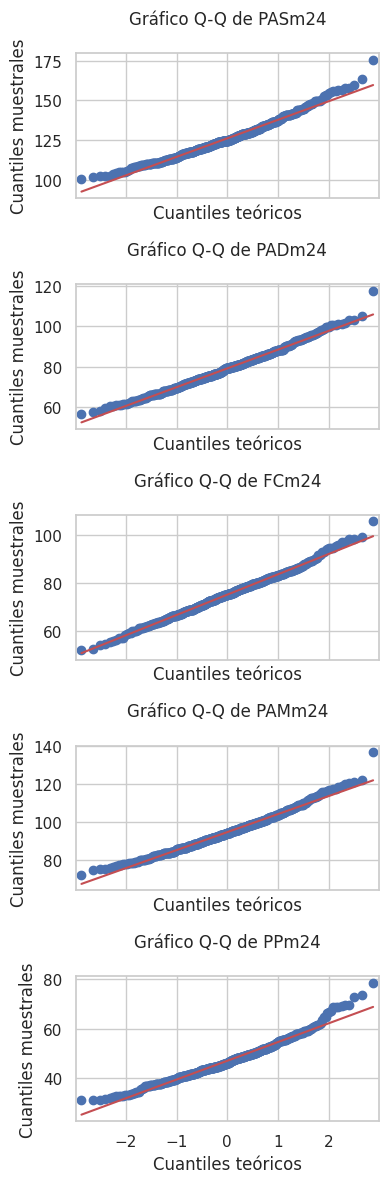
\includegraphics[height=20cm]{./Figures/qqplot_dataset1a.png}}
	\hspace{1em}
	\subcaptionbox{Gráficos Q-Q de las cargas hipertensivas sistólicas y diastólicas \\durante el día y la noche.\label{fig:qqplot_b}}
	[0.45\linewidth]{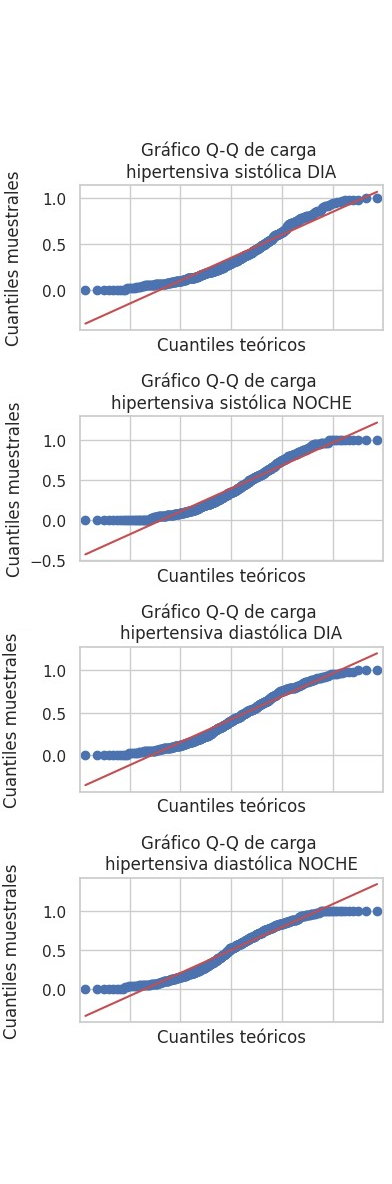
\includegraphics[height=20cm]{./Figures/qqplot_dataset1b.png}}
	\caption{Gráficos Q-Q de variables cuantitativas.}\label{fig:qqplot_1}
\end{figure}

\begin{figure}[H]
	\centering
	\hspace{1em}
	\subcaptionbox{Histogramas de la PAS, PAD, FC, PAM y PP durante 24 h.\label{fig:hist_a}}
	[0.45\linewidth]{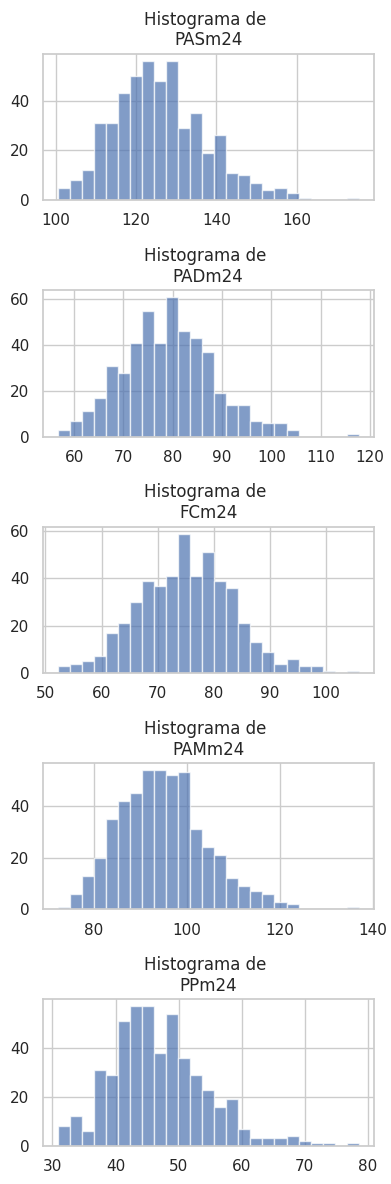
\includegraphics[height=20cm]{./Figures/histograma_dataset1a.png}}
	\hspace{1em}
	\subcaptionbox{Histogramas de las cargas hipertensivas sistólicas y diastólicas durante el día y la noche.\label{fig:hist_b}}
	[0.45\linewidth]{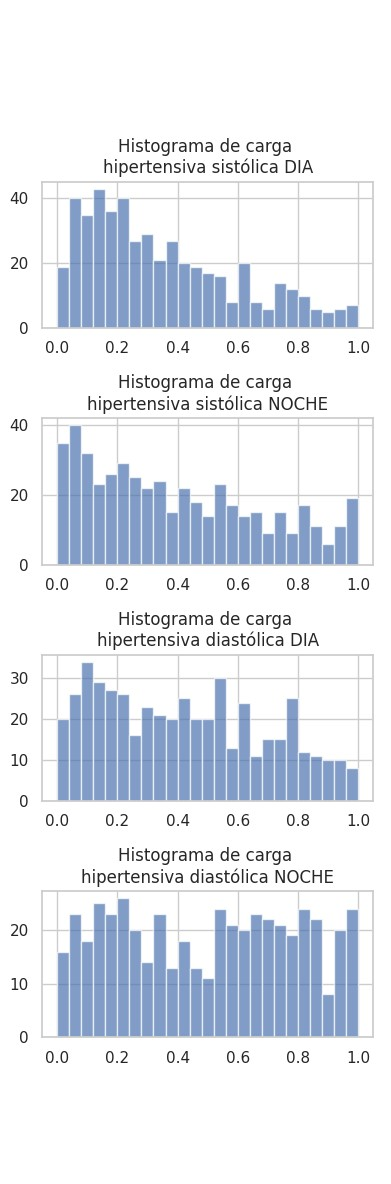
\includegraphics[height=20cm]{./Figures/histograma_dataset1b.png}}
	\caption{Histogramas de variables cuantitativas.}\label{fig:histogram_1}
\end{figure}


%%%%%%%%%%%%%%%%%%%%%%%
%%%%%%%%%%%%%%%%%%%%%%%
%\pagebreak 
%\filbreak 
\subsubsection{Tratamiento de clases desbalanceadas }
En el contexto de este trabajo, se identificó un desbalance de clases, lo cual significa que una de las clases 
está representada por una fracción muy pequeña de las muestras totales. En la figura \ref{fig:desbalance_a} se puede 
observar que solamente un 7.54\% de las muestras pertenecen a la clase positiva, lo que equivale a 37 pacientes con MACE = 1. 
Este desequilibrio en las clases es un fenómeno intrínseco y esperable, ya que refleja la naturaleza del proceso 
que genera los datos. Sin embargo, el desbalance de clases puede crear un sesgo en el modelo de aprendizaje 
automático, ya que tiende a favorecer la predicción de la clase mayoritaria en lugar de capturar adecuadamente 
las instancias de la clase minoritaria. 

Para mitigar este problema, existen diversas técnicas que permiten equilibrar las clases en el conjunto de datos. 
En particular, para este trabajo se empleó la técnica SMOTE, la cual consiste en generar de forma sintética nuevos 
ejemplos de la clase minoritaria. De esta forma, se logró abordar de manera más precisa y equitativa el desafío 
de la predicción en un escenario desbalanceado. El nuevo conjunto de datos balanceado se exhibe en la figura \ref{fig:desbalance_b}.


\begin{figure}[H]
	\centering
	\hspace{1em}
	\subcaptionbox{Conjunto de datos desbalanceado.\label{fig:desbalance_a}}
	[0.45\linewidth]{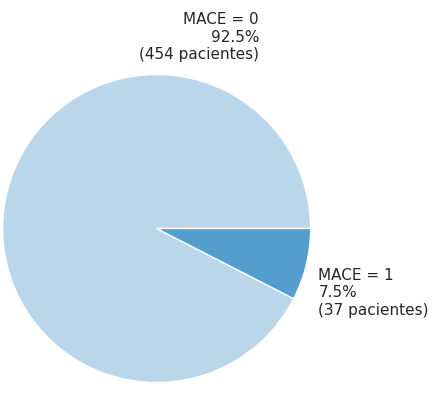
\includegraphics[height=6cm]{./Figures/desbalance_pie.png}}
	\hspace{1em}
	\subcaptionbox{Conjunto de datos después de emplear SMOTE.\label{fig:desbalance_b}}
	[0.45\linewidth]{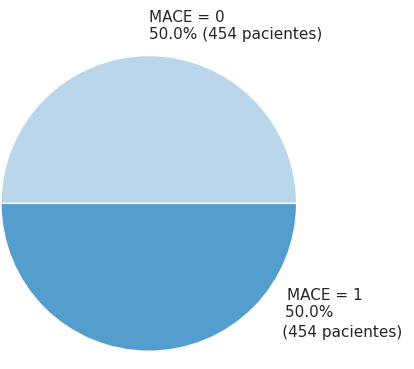
\includegraphics[height=5.5cm]{./Figures/desbalance_smote_pie.png}}
	\caption{Conjunto de datos antes y después de aplicar SMOTE.}
\end{figure}

%%%%%%%%%%%%%%%%%%%%%%%
%%%%%%%%%%%%%%%%%%%%%%%
\subsubsection{Normalización de características}
La normalización de los datos es un paso crucial antes de entrenar una red neuronal, y tiene como 
objetivo principal igualar la escala de las características de entrada. Esto es importante puesto 
que las redes neuronales son sensibles a las diferencias de escala entre las variables. En otras 
palabras, cuando los datos presentan diferentes escalas, algunas características con valores numéricos 
más altos pueden tener un impacto desproporcionado en el proceso de entrenamiento. Esto puede ocasionar 
una mayor influencia en los pesos de la red y distorsionar el modelo resultante. 
Además, las funciones de activación utilizadas en las neuronas pueden funcionar de manera óptima 
cuando los datos están normalizados en un rango adecuado.

En este trabajo, se decidió utilizar el método \emph{StandardScaler} de \emph{scikit-learn} \citep{CITE:50} para 
normalizar las características de entrada. Este método aplica una transformación que ajusta la 
media de cada característica a 0 y la desviación estándar a 1. La definición de la transformación 
se muestra en la ecuación \ref{eq:normalizacion}, donde $X$ representa la matriz de características de 
entrada, $\mu$ a la media y $\sigma$ al desvío estándar. 

\begin{equation}
	\label{eq:normalizacion}
	X_{\text{normalizado}} = \frac{X - \mu}{\sigma}
\end{equation}

Al normalizar los datos de esta manera, se garantiza que todas las características tengan la 
misma escala, lo que facilita el proceso de aprendizaje de la red neuronal y mejora la convergencia 
del modelo. En la figura \ref{fig:normalizacion} se muestran a modo de ejemplo las distribuciones de 
la PAS, PAD y FC medias durante 24 horas antes y después de ser normalizadas. 

\begin{figure}[H]
	\centering
	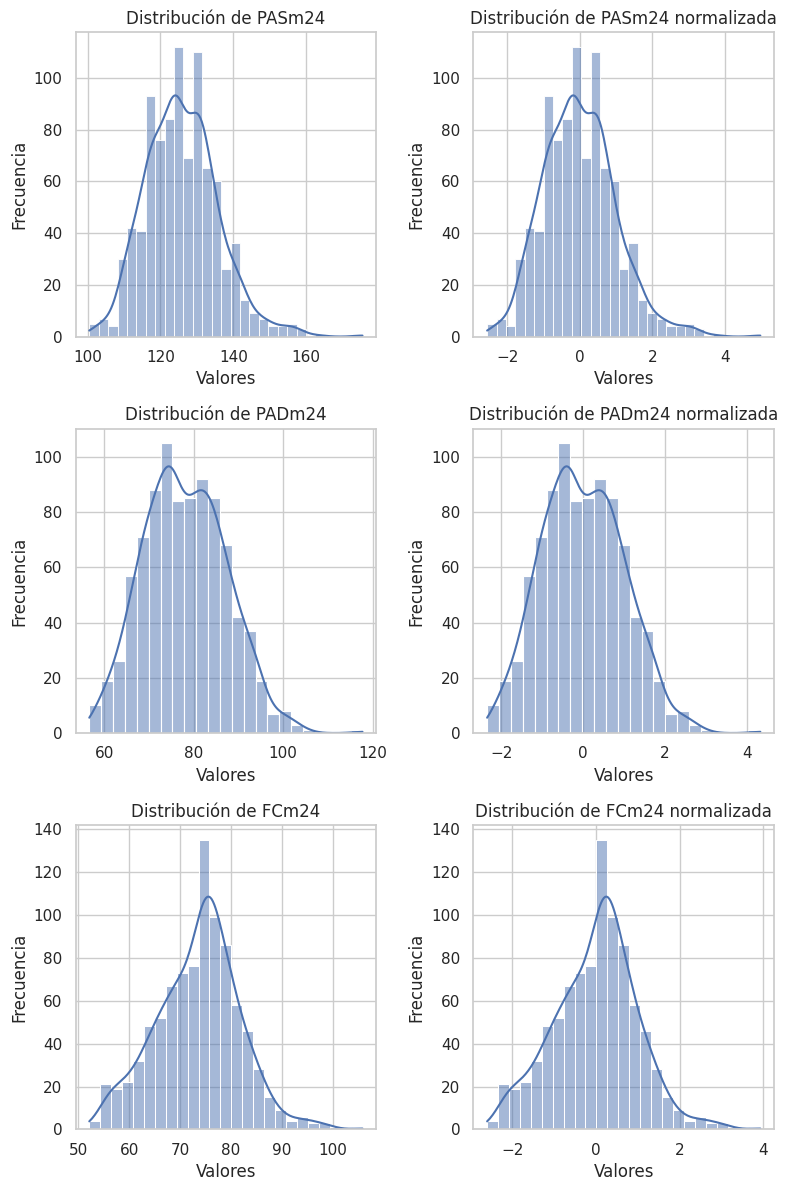
\includegraphics[width=0.8\textwidth]{./Figures/normalizacion.png}
	\caption{Distribuciones de la PAS, PAD y FC durante 24 h \\antes y después de la normalización.}\label{fig:normalizacion}
\end{figure}

%%%%%%%%%%%%%%%%%%%%%%%
%%%%%%%%%%%%%%%%%%%%%%%
\subsubsection{Selección de características}

La selección de variables para un modelo de red neuronal es un proceso crítico que tiene como objetivo 
elegir las variables más relevantes y evitar la inclusión de aquellas que sean redundantes o 
problemáticas. Durante el desarrollo de este trabajo, se identificaron dos variables que son 
combinaciones lineales de otras. Específicamente, se encontró que la presión arterial media y 
la presión de pulso dependen linealmente de la presión arterial sistólica y diastólica. 
Esta relación se definió matemáticamente en la subsección \ref{IntroPresiones} y 
se puede visualizar claramente en la figura \ref{fig:pamypp}. 

\begin{figure}[H]
	\centering
	\hspace{1em}
	\subcaptionbox{Relación lineal de PAM con PAS y PAD.\label{fig:pam}}
	[0.45\linewidth]{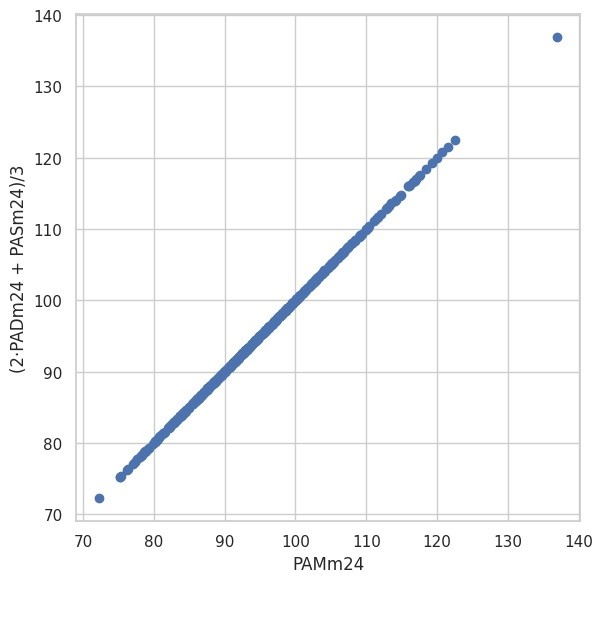
\includegraphics[height=6.5cm]{./Figures/PAM.jpg}}
	\hspace{1em}
	\subcaptionbox{Relación lineal de PP con PAS y PAD.\label{fig:pp}}
	[0.45\linewidth]{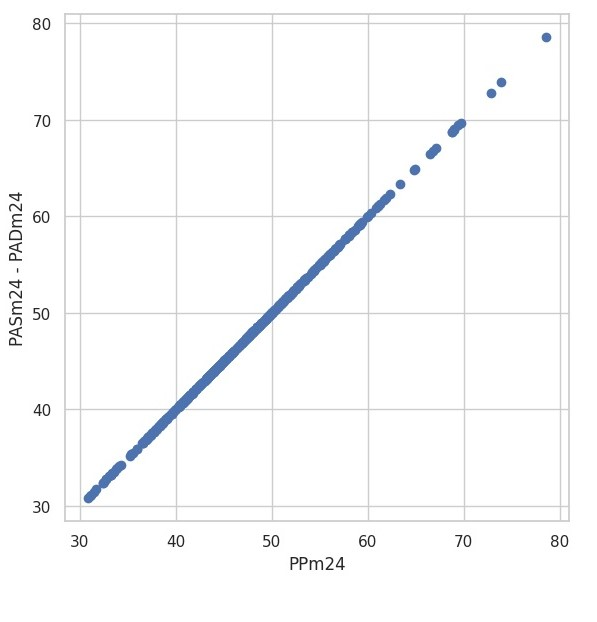
\includegraphics[height=6.5cm]{./Figures/PP.jpg}}
	\caption{Combinaciones lineales de la presión arterial media y presión de pulso con las presiones sistólicas y diastólicas.}\label{fig:pamypp}
\end{figure}


Teniendo en consideración esta información, se tomó la decisión de no incluir estas variables en 
la red neuronal por diversos motivos. En primer lugar, se buscó evitar la redundancia de información. 
Si una variable es una combinación lineal de otras, significa que la información contenida en 
dicha variable ya está presente en las demás. Por lo tanto, su inclusión solo duplicaría la 
información en la red neuronal, lo cual genera una sobrecarga y ralentiza el proceso de 
entrenamiento. Además, es posible que se generen problemas de inestabilidad numérica puesto que incluso 
pequeñas variaciones en los valores de entrada pueden dar lugar a variaciones significativas 
en las salidas. Esto podría comprometer la estabilidad y precisión de la red neuronal, afectando 
negativamente su rendimiento y capacidad de generar resultados confiables. Otro motivo para 
excluir estas variables es evitar que el modelo se ajuste en exceso a los datos de entrenamiento. 
Es posible que esto resulte en una pérdida de generalización, lo que significa que la red tendría 
dificultades para adaptarse a nuevos datos no vistos anteriormente.

En consecuencia, para abordar estos problemas, se decidió eliminar los valores medios y desviaciones 
estándar de PAM y PP. Así, se preservaron únicamente los valores medidos por el presurómetro: la PAS y PAD. 
De este modo, se asegura que la red neuronal se enfoque en las variables fundamentales y se evitan 
los problemas mencionados anteriormente.

Por otro lado, las variables que incluyen fechas son útiles para brindar fiabilidad a 
la base de datos, ya que proporcionan información sobre el momento en el que se realizó el MAPA y, en caso 
de que hubiese ocurrido, el momento en el que se produjo un evento.
Sin embargo, en el contexto de predecir MACE, estas variables pueden considerarse irrelevantes ya 
que no aportan información sustancial para predecir el resultado deseado. En otras palabras, 
la fecha en sí misma no contiene información directa sobre los atributos fisiológicos o clínicos 
que están más relacionados con la ocurrencia de MACE. Además de su falta de 
relevancia, mantener la variable de fecha agregaría una complejidad adicional al modelo 
de red neuronal. La representación y codificación de la fecha como una característica en el 
modelo requiere un procesamiento adicional. Su transformación en valores numéricos o la 
creación de variables categóricas adicionales aumentaría la dimensionalidad de los datos 
y podría dificultar la interpretación de la red neuronal. Por lo tanto, se decidió eliminar 
esta variable con el fin de agilizar el análisis y entrenamiento de la red neuronal. 

Después de realizar el preprocesamiento a la información proveniente del MAPA, el conjunto 
de datos final utilizado para el desarrollo del modelo incluye las siguientes variables de entrada:

\begin{itemize}
	\item PASm24	
  \item PADm24
  \item FCm24
  \item PASsd24 
  \item PADsd24
  \item FCsd24
  \item PASmDIA
  \item PADmDIA
  \item FCmDIA
  \item htaloadsbpDIA 
  \item htaloaddbpDIA   
  \item HTAdia01	
  \item PASmNOCHE
  \item PADmNOCHE
  \item FCmNOCHE
  \item htaloadsbpNOCHE
  \item htaloaddbpNOCHE
  \item HTAnoche01
\end{itemize}


%%%%%%%%%%%%%%%%%%%%%%%%%%%%%%%%%%%%%%%%%%%%%%%%%%%%%%%%%%%%%%%%%%%%%%%%%%%%%%%%%%%%%%%%%%%%
%%%%%%%%%%%%%%%%%%%%%%%%%%%%%%%%%%%%%%%%%%%%%%%%%%%%%%%%%%%%%%%%%%%%%%%%%%%%%%%%%%%%%%%%%%%%
%------------------------------------------------------------------------
%	datos presurometrias + datos clinicos
\subsection{Conjunto de datos de presurometrías y datos clínicos}
\label{sec:Conjunto2}

El segundo conjunto de datos utilizado incorpora los datos clínicos adicionales de los 491 pacientes que 
se realizaron el MAPA, complementando así la información del conjunto de datos anterior. Dado que muchas 
de las variables son las mismas, esta subsección se enfoca exclusivamente en el preprocesamiento aplicado 
a las nuevas variables clínicas. Estas incluyen 4 variables numéricas (talla, peso, IMC y edad) y 5 variables 
categóricas (sexo, diabetes, tabaquismo, dislipemia e hipertrofia ventricular izquierda).


%%%%%%%%%%%%%%%%%%%%%%%
%%%%%%%%%%%%%%%%%%%%%%%
\subsubsection{Distribuciones de las variables numéricas}
Para analizar las variables clínicas numéricas del conjunto de datos, se llevaron a cabo pruebas visuales y 
estadísticas. En la figura \ref{fig:qqplots2} se exhiben los gráficos Q-Q e histogramas para las variables 
de interés. En cuanto a la talla, se observó que los datos siguen una distribución aproximadamente normal. 
Tanto el gráfico Q-Q como el histograma mostraron una forma de campana característica de esta distribución. 
En el caso del peso y el IMC, se encontró una distribución asimétrica positiva. Esto indica que hay una mayor 
concentración de valores más bajos y una dispersión hacia valores más altos. Esto se debe a que la media y la 
mediana del peso fueron de 76 kg, mientras que la moda se situó en 85 kg. Dado que el IMC se calcula a partir 
del peso y la talla, su distribución sigue una tendencia similar a la del peso. Por otro lado, en cuanto a 
la variable de edad, se identificó una distribución asimétrica negativa. Esto sugiere que existe una mayor 
cantidad de personas mayores en el conjunto de datos. La media de la edad fue de 65 años, con una edad mínima 
de 19 años y una máxima de 98 años. La moda de la distribución se encontró en 72 años.

\begin{figure}[H]
	\centering
	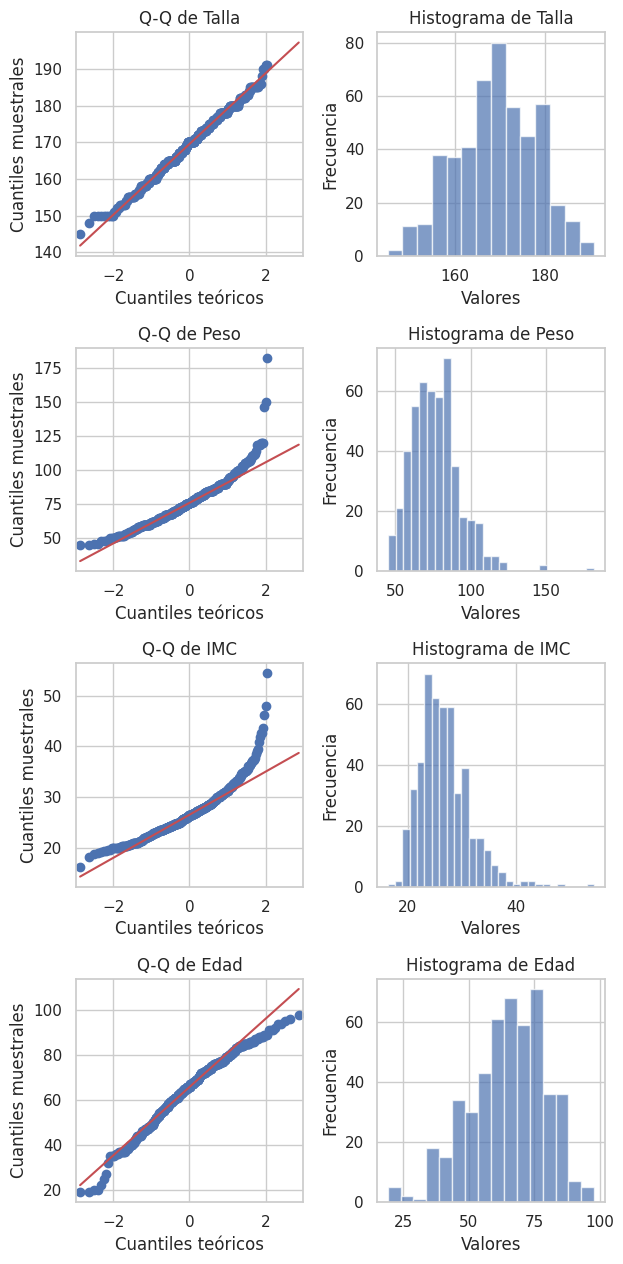
\includegraphics[width=0.8\textwidth]{./Figures/qqplots2.png}
	\caption{Gráficos Q-Q e histogramas de la talla, peso, IMC y edad.}\label{fig:qqplots2}
\end{figure}

Además de los análisis visuales, se realizaron pruebas estadísticas, incluyendo los tests de Shapiro-Wilk 
y Kolmogorov-Smirnov. Los resultados de ambas pruebas indicaron que la talla, el peso y el IMC siguen una 
distribución normal, mientras que la edad no presenta una distribución normal.

%%%%%%%%%%%%%%%%%%%%%%%
%%%%%%%%%%%%%%%%%%%%%%%
%\pagebreak 
\subsubsection{Imputación de valores faltantes}
En el segundo conjunto de datos utilizado, se identificaron diferentes variables con valores faltantes. 
A continuación, se detalla la cantidad de valores ausentes en cada una de estas variables:

\begin{itemize}
  \item Sexo: 1 paciente sin información.
  \item Talla, peso e IMC: 9 pacientes sin datos de talla ni peso, lo cual implica la ausencia del cálculo del IMC.
  \item Dislipemia: 1 paciente sin información.
  \item HVI (hipertrofia ventricular izquierda): 2 pacientes sin información.
\end{itemize}

Ante la presencia de estos valores faltantes, es necesario aplicar técnicas de imputación para completar 
la información y garantizar la integridad de los datos. En este trabajo, se optó por utilizar el método 
\emph{KNNImputer} de \emph{scikit-learn} \citep{CITE:50}. Esta elección se basa en la capacidad del método
para capturar la estructura de los datos y aprovechar la información de las instancias vecinas para la 
imputación. Además, este método es adecuado para manejar variables numéricas y categóricas, lo cual es 
relevante en el contexto de este trabajo.

La imputación de datos faltantes utilizando técnicas como el \emph{KNNImputer} desempeña un papel fundamental 
al minimizar la pérdida de información en conjuntos de datos relativamente pequeños, 
como es el caso de este trabajo. De esta manera, se maximiza la utilidad de los datos disponibles y se evita la exclusión 
de observaciones valiosas debido a la falta de información.

%%%%%%%%%%%%%%%%%%%%%%%
%%%%%%%%%%%%%%%%%%%%%%%

\subsubsection{Tratamiento de clases desbalanceadas}

En relación al tratamiento de desbalance de clases, se aplicó el mismo enfoque que en la subsección 
\ref{sec:Conjunto1} debido a que la variable de salida es la misma. Se utilizó la técnica de sobremuestreo 
SMOTE para abordar el desequilibrio de clases y mejorar la representación de la clase minoritaria en el conjunto de datos. 

%%%%%%%%%%%%%%%%%%%%%%%
%%%%%%%%%%%%%%%%%%%%%%%
\subsubsection{Normalización de características}

Para asegurar que todas las características tengan una escala uniforme, se llevó a cabo un proceso de normalización 
de los datos. Al igual que en la subsección \ref{sec:Conjunto1}, se utilizó el método \emph{StandardScaler} \citep{CITE:50}. La 
figura \ref{fig:normalizacion2} presenta las distribuciones antes y después de la normalización de las variables talla, peso, IMC y edad. Este procedimiento garantiza que todas las variables estén en una escala comparable, 
lo que facilita la interpretación y el análisis de los datos para la red neuronal.

\begin{figure}[H]
	\centering
	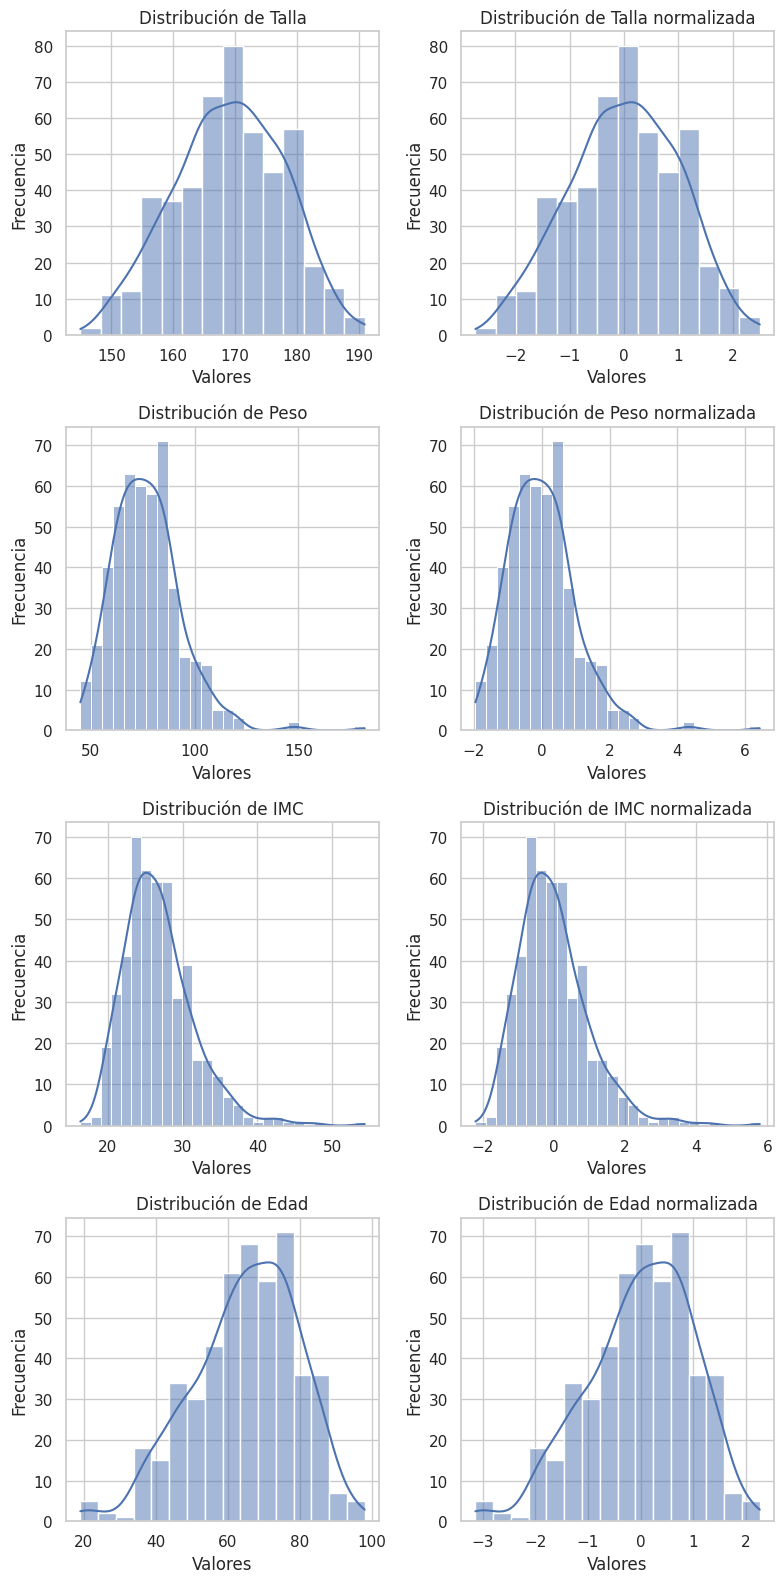
\includegraphics[width=0.7\textwidth]{./Figures/normalizacion2.png}
	\caption{Distribuciones de la talla, peso, IMC y edad antes y después de la normalización.}\label{fig:normalizacion2}
\end{figure}

Después de realizar el preprocesamiento a la información proveniente del MAPA y los datos clínicos, el segundo conjunto de 
datos utilizado para el desarrollo del modelo incluye las siguientes variables de entrada:

\begin{itemize}
  \item PASm24	
  \item PADm24
  \item FCm24
  \item PASsd24 
  \item PADsd24
  \item FCsd24
  \item PASmDIA
  \item PADmDIA
  \item FCmDIA
  \item htaloadsbpDIA 
  \item htaloaddbpDIA   
  \item HTAdia01	
  \item PASmNOCHE
  \item PADmNOCHE
  \item FCmNOCHE
  \item htaloadsbpNOCHE
  \item htaloaddbpNOCHE
  \item HTAnoche01
  \item Talla
  \item Peso
  \item IMC
  \item Edad
  \item Sexo
  \item DBT
  \item Tabaquismo
  \item Dislipemia
  \item HVI
\end{itemize}

%------------------------------------------------------------------------
%	DISEÑO Y DESARROLLO DE MODELOS
%----------------------------------------------------------------------------------------
\section{Diseño y desarrollo de modelos}
El proceso de diseño e implementación de los modelos se llevó a cabo de igual manera para ambos 
conjuntos de datos. A continuación, se presentan en detalle las métricas utilizadas, la 
arquitectura de los modelos y el proceso de entrenamiento.

%%%%%%%%%%%%%%%%%%%%%%%%%%%%%%%%%%%%%%%%%%%%%%%%%%%%%%%%%%%%%%%%%%%%%%%%%%%%%%%%%%%%%%%%%%%%
%%%%%%%%%%%%%%%%%%%%%%%%%%%%%%%%%%%%%%%%%%%%%%%%%%%%%%%%%%%%%%%%%%%%%%%%%%%%%%%%%%%%%%%%%%%%
%------------------------------------------------------------------------
%	Definición de métricas
\subsection{Definición de métricas}

Para evaluar el desempeño de los modelos de forma objetiva, se empleó la métrica AUC. La curva ROC y, 
en particular, el AUC son ampliamente utilizados en la evaluación de modelos de clasificación para 
medir la capacidad de distinguir entre clases positivas y negativas. Para este trabajo en particular, 
la elección se debe a la relevancia clínica de analizar la relación entre la sensibilidad y especificidad. 
En otras palabras, se buscó un equilibrio óptimo entre la detección temprana de casos positivos de MACE 
y la minimización de falsas alarmas. Además, la solicitud específica del cliente de lograr un AUC superior 
al 85\% justificó el uso del AUC como métrica clave. 

A su vez, el servicio de cardiología del Hospital Alemán enfatizó la importancia de evitar falsos negativos. 
Esto implicó que se priorizara la correcta clasificación de casos positivos aunque esto signifique un aumento 
en la tasa de falsos positivos y una posible reducción en otras métricas de evaluación. 

Por otro lado, se calcularon otras métricas además del AUC como \emph{precision}, \emph{recall} y \emph{accuracy} 
para obtener una visión más completa de los resultados del modelo.


%%%%%%%%%%%%%%%%%%%%%%%%%%%%%%%%%%%%%%%%%%%%%%%%%%%%%%%%%%%%%%%%%%%%%%%%%%%%%%%%%%%%%%%%%%%%
%%%%%%%%%%%%%%%%%%%%%%%%%%%%%%%%%%%%%%%%%%%%%%%%%%%%%%%%%%%%%%%%%%%%%%%%%%%%%%%%%%%%%%%%%%%%
%------------------------------------------------------------------------
%	Arquitectura de los modelos
\subsection{Arquitectura de los modelos}
Una vez definido el objetivo del modelo y preprocesados los datos, se seleccionó la arquitectura básica del modelo. 
Se decidió emplear un perceptron multicapa puesto que permite capturar relaciones y patrones no lineales en los 
datos. Además, los MLP tienen gran flexibilidad en la representación de características y enorme capacidad para 
aprender representaciones más abstractas y de mayor nivel. De este modo, esta arquitectura puede llevar a una 
mejor habilidad de generalización \citep{CITE:35} \citep{CITE:44}. 

%%%%%%%%%%%%%%%%%%%%%%%
%%%%%%%%%%%%%%%%%%%%%%%
\subsubsection{Definición de la estructura de capas}
Se llevó a cabo una investigación exhaustiva para determinar la configuración óptima del modelo, incluyendo el 
número de capas ocultas y la cantidad de neuronas en cada capa. Dado que no se disponía de conocimientos previos 
sobre la arquitectura ideal, se realizó una búsqueda sistemática de hiperparámetros. Se consideraron diferentes 
alternativas, como 1, 2, 3 o 4 capas ocultas, y se establecieron múltiples opciones para el número de neuronas 
en la primera capa oculta, incluyendo 10, 20, 30, 40 o 50 nodos. En caso de tener múltiples capas ocultas, se 
decidió que la cantidad de neuronas en las capas posteriores fuese la mitad de las de la capa anterior. 
La tabla \ref{tab:tablamodelos} muestra las diferentes combinaciones de modelos que resultaron de esta exploración.


\begin{table}[H]
	\centering
	\caption[Configuraciones de modelos explorados]{Configuraciones de modelos explorados con la cantidad de neuronas por capa oculta.}
	\begin{tabular}{l c c c c}    
		\toprule
		\textbf{Modelo} & \textbf{Capa 1} & \textbf{Capa 2} & \textbf{Capa 3} & \textbf{Capa 4} \\
		\midrule
    \multicolumn{5}{c}{1 capa oculta} \\
    \hline
		1                & 50             & -			          & -               & -	\\
    2                & 40             & -			          & -               & -	\\
    3                & 30             & -			          & -               & -	\\
    4                & 20             & -			          & -               & -	\\
    5                & 10             & -			          & -               & -	\\

    \hline
    \multicolumn{5}{c}{2 capas ocultas} \\
    \hline

    6                & 50             & 25			        & -               & -	\\
    7                & 40             & 20			        & -               & -	\\
    8                & 30             & 15			        & -               & -	\\
    9                & 20             & 10			        & -               & -	\\
    10               & 10             & 5			          & -               & -	\\

    \hline
    \multicolumn{5}{c}{3 capas ocultas} \\
    \hline

    11               & 50             & 25			        & 12              & -	\\
    12               & 40             & 20			        & 10              & -	\\
    13               & 30             & 15			        & 7               & -	\\
    14               & 20             & 10			        & 5               & -	\\
    15               & 10             & 5			          & 2               & -	\\

    \hline
    \multicolumn{5}{c}{4 capas ocultas} \\
    \hline

    16               & 50             & 25			        & 12              & 6	\\
    17               & 40             & 20			        & 10              & 5	\\
    18               & 30             & 15			        & 7               & 3	\\
    19               & 20             & 10			        & 5               & 2	\\
    20               & 10             & 5			          & 2               & 1	\\

		\bottomrule
		\hline
	\end{tabular}
	\label{tab:tablamodelos}
\end{table}

La figura \ref{fig:AUC_exploracion_dataset} muestra los valores promedio de AUC obtenidos 
mediante $k=5$ iteraciones de validación cruzada para los modelos presentados en la tabla \ref{tab:tablamodelos}. 
Se observa que, en el caso del conjunto de datos de presurometrías, los tres modelos con el mejor rendimiento 
en términos de AUC presentan una arquitectura de dos capas ocultas, donde la primera capa cuenta con 30 o más 
nodos (modelos 6, 7 y 8 de la tabla \ref{tab:tablamodelos}). En contraste, para el conjunto de datos que incluye 
información clínica, se encontró que el mejor desempeño en términos de AUC se logró con un modelo de una sola 
capa oculta, con 30 o más nodos en la primera capa (modelos 1, 2 y 3 de la tabla \ref{tab:tablamodelos}).

\begin{figure}[H]
	\centering
	\hspace{1em}
	\subcaptionbox{Valores promedio de AUC obtenidos para el conjunto de datos de MAPA.\label{fig:AUC_exploracion_dataset1}}
	{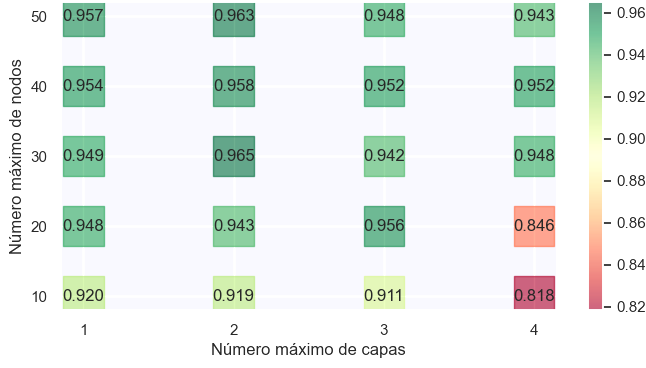
\includegraphics[width=0.96\textwidth]{./Figures/AUC_exploracion_dataset1.png}}
	\hspace{1em}
	\subcaptionbox{Valores promedio de AUC obtenidos para el conjunto de datos de MAPA y datos clínicos.\label{fig:AUC_exploracion_dataset2}}
	{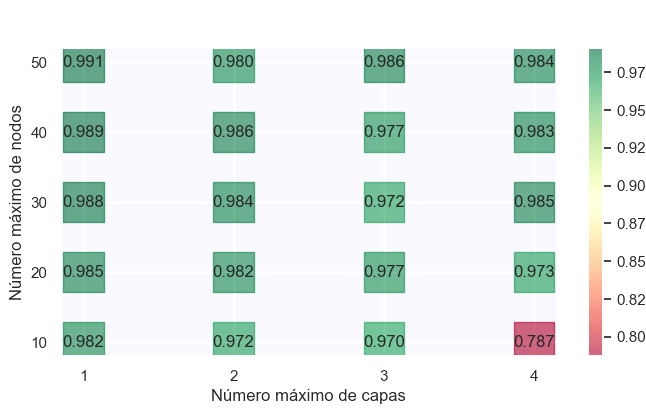
\includegraphics[width=0.96\textwidth]{./Figures/AUC_exploracion_dataset2.png}}
	\caption[Valores promedio de AUC obtenidos mediante $k=5$ iteraciones de validación cruzada.]{Valores promedio de AUC obtenidos mediante $k=5$ iteraciones de validación cruzada para los modelos evaluados.}\label{fig:AUC_exploracion_dataset}
\end{figure}

Con base en los hallazgos anteriores, se llevó a cabo una búsqueda más exhaustiva para determinar la 
arquitectura óptima del modelo. Para el primer conjunto de datos, se realizaron pruebas con modelos 
que incluían dos capas ocultas, explorando diferentes combinaciones. La primera capa se configuró 
con un rango de 20 a 50 nodos, incrementando de uno en uno, mientras que la segunda capa se definió 
con la mitad de las neuronas de la primera capa, es decir, de 10 a 25 nodos, también en incrementos 
de uno. Los resultados obtenidos para cada configuración se registraron en la tabla \ref{tab:tablamodelos_2layers}. 
Por otro lado, para el conjunto de datos que incluía variables clínicas adicionales, se realizó una 
búsqueda de la cantidad de nodos óptima para la capa oculta, dentro de un rango de 30 a 55, con un 
incremento de un nodo. Los resultados de esta exploración se presentan en la tabla \ref{tab:tablamodelos_2layers}.

\begin{table}[H]
	\centering
	\caption[Configuraciones de modelos explorados]{Configuraciones de modelos explorados con la cantidad de neuronas por capa oculta.}
	\begin{tabular}{l c c c c c c}    
		\toprule
		\textbf{Modelo} & \textbf{Capa 1} & \textbf{Capa 2} & \textbf{\emph{Accuracy}} & \textbf{\emph{Precision}} & \textbf{\emph{Recall}}  & \textbf{AUC}\\
		\midrule
    
      1 & 50 & 25	& 0.935 $\pm$ 0.021 & 0.902  $\pm$ 0.037	& 0.977  $\pm$ 0.014 & 0.968  $\pm$ 0.016\\
      2 & 49 & 24 & 0.930 $\pm$ 0.026 & 0.900  $\pm$ 0.044 & 0.971  $\pm$ 0.005 & 0.964 $\pm$ 0.010\\
      3 & 48 & 24 & 0.931 $\pm$ 0.022 & 0.901 $\pm$ 0.033 & 0.971 $\pm$ 0.011 & 0.967 $\pm$ 0.009\\
      4 & 47 & 23 & 0.924 $\pm$ 0.017 & 0.890 $\pm$ 0.028 & 0.971 $\pm$ 0.015 & 0.963 $\pm$ 0.008\\
      5 & 46 & 23 & 0.922 $\pm$ 0.025 & 0.888 $\pm$ 0.040 & 0.968 $\pm$ 0.011 & 0.953 $\pm$ 0.011\\
      6 & 45 & 22 & 0.924 $\pm$ 0.024 & 0.889 $\pm$ 0.041 & 0.973 $\pm$ 0.009 & 0.961 $\pm$ 0.011\\ 
      7 & 44 & 22 & 0.921 $\pm$ 0.019 & 0.877 $\pm$ 0.034 & 0.982 $\pm$ 0.015 & 0.958 $\pm$ 0.016\\ 
      8 & 43 & 21 & 0.933 $\pm$ 0.017 & 0.902 $\pm$ 0.025 & 0.973 $\pm$ 0.009 & 0.963 $\pm$ 0.012\\ 
      9 & 42 & 21 & 0.922 $\pm$ 0.015 & 0.887 $\pm$ 0.021 & 0.968 $\pm$ 0.004 & 0.962 $\pm$ 0.010\\ 
      10 & 41 & 20 & 0.920 $\pm$ 0.021 & 0.881 $\pm$ 0.034 & 0.973 $\pm$ 0.011 & 0.961 $\pm$ 0.011\\ 
      11 & 40 & 20 & 0.920 $\pm$ 0.028 & 0.880 $\pm$ 0.049 & 0.977 $\pm$ 0.014 & 0.958 $\pm$ 0.017\\ 
      12 & 39 & 19 & 0.923 $\pm$ 0.024 & 0.891 $\pm$ 0.033 & 0.966 $\pm$ 0.014 & 0.961 $\pm$ 0.015\\ 
      13 & 38 & 19 & 0.923 $\pm$ 0.022 & 0.888 $\pm$ 0.036 & 0.971 $\pm$ 0.011 & 0.956 $\pm$ 0.009\\ 
      14 & 37 & 18 & 0.929 $\pm$ 0.012 & 0.898 $\pm$ 0.024 & 0.968 $\pm$ 0.013 & 0.964 $\pm$ 0.012\\ 
      15 & 36 & 18 & 0.928 $\pm$ 0.016 & 0.899 $\pm$ 0.032 & 0.966 $\pm$ 0.012 & 0.960 $\pm$ 0.006\\ 
      16 & 35 & 17 & 0.925 $\pm$ 0.023 & 0.899 $\pm$ 0.041 & 0.962 $\pm$ 0.006 & 0.960 $\pm$ 0.012\\ 
      17 & 34 & 17 & 0.910 $\pm$ 0.008 & 0.866 $\pm$ 0.018 & 0.971 $\pm$ 0.017 & 0.940 $\pm$ 0.011\\ 
      18 & 33 & 16 & 0.920 $\pm$ 0.014 & 0.885 $\pm$ 0.022 & 0.966 $\pm$ 0.007 & 0.965 $\pm$ 0.013\\ 
      19 & 32 & 16 & 0.921 $\pm$ 0.012 & 0.885 $\pm$ 0.021 & 0.968 $\pm$ 0.013 & 0.959 $\pm$ 0.011\\ 
      20 & 31 & 15 & 0.920 $\pm$ 0.020 & 0.881 $\pm$ 0.030 & 0.973 $\pm$ 0.013 & 0.959 $\pm$ 0.009\\ 
      21 & 30 & 15 & 0.921 $\pm$ 0.017 & 0.889 $\pm$ 0.028 & 0.964 $\pm$ 0.011 & 0.959 $\pm$ 0.012\\ 
      22 & 29 & 14 & 0.923 $\pm$ 0.020 & 0.891 $\pm$ 0.031 & 0.966 $\pm$ 0.007 & 0.961 $\pm$ 0.016\\ 
      23 & 28 & 14 & 0.930 $\pm$ 0.034 & 0.901 $\pm$ 0.053 & 0.971 $\pm$ 0.014 & 0.965 $\pm$ 0.021\\ 
      24 & 27 & 13 & 0.920 $\pm$ 0.027 & 0.887 $\pm$ 0.046 & 0.966 $\pm$ 0.016 & 0.957 $\pm$ 0.012\\ 
      25 & 26 & 13 & 0.909 $\pm$ 0.023 & 0.868 $\pm$ 0.037 & 0.966 $\pm$ 0.016 & 0.953 $\pm$ 0.019\\ 
      26 & 25 & 12 & 0.922 $\pm$ 0.014 & 0.887 $\pm$ 0.025 & 0.969 $\pm$ 0.027 & 0.957 $\pm$ 0.012\\ 
      27 & 24 & 12 & 0.916 $\pm$ 0.013 & 0.878 $\pm$ 0.021 & 0.968 $\pm$ 0.008 & 0.952 $\pm$ 0.010\\ 
      28 & 23 & 11 & 0.919 $\pm$ 0.017 & 0.884 $\pm$ 0.028 & 0.966 $\pm$ 0.012 & 0.950 $\pm$ 0.015\\ 
      29 & 22 & 11 & 0.920 $\pm$ 0.019 & 0.885 $\pm$ 0.027 & 0.966 $\pm$ 0.007 & 0.953 $\pm$ 0.013\\ 
      30 & 21 & 10 & 0.916 $\pm$ 0.011 & 0.878 $\pm$ 0.022 & 0.968 $\pm$ 0.013 & 0.954 $\pm$ 0.013\\ 
      31 & 20 & 10 & 0.920 $\pm$ 0.023 & 0.884 $\pm$ 0.035 & 0.968 $\pm$ 0.017 & 0.945 $\pm$ 0.026\\
      
		\bottomrule
		\hline
	\end{tabular}
	\label{tab:tablamodelos_2layers}
\end{table}

%%%%%%%%%%%%%%%%%%%%%%%%%%%%%%%%%%%%%%%%%%%%
%%%%%%%%%%%%%%%%%%%%%%%%%%%%%%%%%%%%%%%%%%%%
%% AGREGAR!
%%%%FALTA AGREGAR LA TABLA DEL DATASET 2%%%%
%%%%%%%%%%%%%%%%%%%%%%%%%%%%%%%%%%%%%%%%%%%%
%%%%%%%%%%%%%%%%%%%%%%%%%%%%%%%%%%%%%%%%%%%

La figura \ref{fig:arquitectura_datasets} muestra la arquitectura final utilizada para cada conjunto de datos. 
Se observa que se optó por una estructura basada en capas densas, también conocidas como capas 
completamente conectadas, complementadas con capas de \emph{dropout}. La incorporación de las capas 
densas permitió capturar relaciones complejas presentes en los datos, mientras que las capas de 
\emph{dropout} desempeñaron un papel fundamental en la regularización del modelo y en la prevención 
del sobreajuste. Como resultado, se logró obtener un modelo con una mayor capacidad de generalización 
y un mejor desempeño en la predicción de datos desconocidos.


\begin{figure}[H]
	\centering
	\hspace{1em}
	\subcaptionbox{Arquitectura del modelo para el conjunto de datos de MAPA.\label{fig:arquitectura_dataset1}}
	{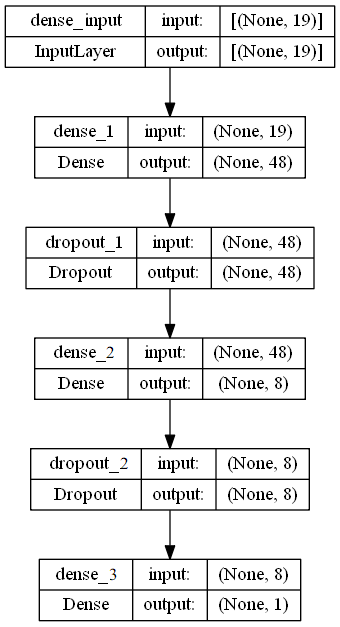
\includegraphics[width=0.45\textwidth]{./Figures/arquitectura_dataset1.png}}
	\hspace{1em}
	\subcaptionbox{Arquitectura del modelo para el conjunto de datos de MAPA y datos clínicos.\label{fig:arquitectura_dataset2}}
	{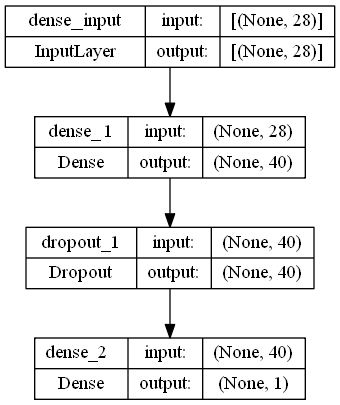
\includegraphics[width=0.45\textwidth]{./Figures/arquitectura_dataset2.png}}
	\caption{Arquitectura elegida para los modelos.}\label{fig:arquitectura_datasets}
\end{figure}

%%%%%%%%%%%%%%%%%%%%%%%
%%%%%%%%%%%%%%%%%%%%%%%
\subsubsection{Selección de funciones de activación, función de pérdida y algoritmo de optimización}
Se empleó la función de activación ReLU en las capas ocultas de la red neuronal. Esta función es 
comúnmente elegida debido a su capacidad para introducir no linealidad en el modelo y capturar 
patrones complejos en los datos. Además, se utilizó la función de activación sigmoide en la capa 
de salida, ya que el problema abordado se trata de una clasificación binaria. La función sigmoide
 es adecuada en este contexto, considerando que mapea los valores de salida a un rango entre 0 y 1, 
 lo que se interpreta como la probabilidad de pertenecer a una de las dos clases posibles.

 Por otro lado, se optó por utilizar la función de pérdida \emph{binary cross entropy} debido a 
 que el problema en cuestión involucra una clasificación binaria. Esta función de pérdida es 
 adecuada para este tipo de problemas, ya que penaliza de manera efectiva las discrepancias 
 entre las predicciones del modelo y los valores reales. En cuanto al algoritmo de optimización, 
 se eligió Adam debido a su eficiencia en la convergencia y adaptabilidad a diferentes tasas de 
 aprendizaje, cómo se explicó en la subsección \ref{sec:optimizador}.

%%%%%%%%%%%%%%%%%%%%%%%
%%%%%%%%%%%%%%%%%%%%%%%
%% AGREGAR!
%AGREGAR ACA LA MODIFICACION A LA FUNCIÓN DE PERDIDA Y CURVAS DE PARETO?
%%%%%%%%%%%%%%%%%%%%%%%
%%%%%%%%%%%%%%%%%%%%%%%



%%%%%%%%%%%%%%%%%%%%%%%
%%%%%%%%%%%%%%%%%%%%%%%
\subsubsection{Selección de hiperparámetros}

Una vez definida la arquitectura inicial de la red neuronal, se realizó una búsqueda de hiperparámetros 
adicionales utilizando el enfoque de búsqueda aleatoria, también conocido cómo \emph{RandomSearch} \citep{CITE:50}. 
Esto se combinó con una validación cruzada de $k=5$ iteraciones para evaluar el rendimiento del modelo en diferentes 
conjuntos de datos y asegurar que los hiperparámetros ajustados generalicen bien. Este ajuste tuvo como objetivo 
encontrar el equilibrio adecuado entre el rendimiento del modelo y la capacidad de generalización. 

%%%%%%%%%%%%%%%%%%%%%%%
%%%%%%%%%%%%%%%%%%%%%%%
%% AGREGAR!
%La tabla \ref{} muestra los hiperparámetros ajustados, los rangos de búsqueda aleatoria y los mejores resultados 
%obtenidos para el conjunto de datos de presurometrías. Por otro lado, la tabla \ref{X2} presenta la misma información 
%para el conjunto de datos que incluye datos clínicos.
%% Chapter Template

\chapter{Ensayos y resultados} % Main chapter title

\label{Chapter4} % Change X to a consecutive number; for referencing this chapter elsewhere, use \ref{ChapterX}

%----------------------------------------------------------------------------------------
%	SECTION 1
%----------------------------------------------------------------------------------------

\section{Pruebas funcionales del hardware}
\label{sec:pruebasHW}

La idea de esta sección es explicar cómo se hicieron los ensayos, qué resultados se obtuvieron y analizarlos.
 
%% Chapter Template

\chapter{Conclusiones} % Main chapter title

\label{Chapter5} % Change X to a consecutive number; for referencing this chapter elsewhere, use \ref{ChapterX}


%----------------------------------------------------------------------------------------

%----------------------------------------------------------------------------------------
%	SECTION 1
%----------------------------------------------------------------------------------------

\section{Conclusiones generales }

La idea de esta sección es resaltar cuáles son los principales aportes del trabajo realizado y cómo se podría continuar. Debe ser especialmente breve y concisa. Es buena idea usar un listado para enumerar los logros obtenidos.

Algunas preguntas que pueden servir para completar este capítulo:

\begin{itemize}
\item ¿Cuál es el grado de cumplimiento de los requerimientos?
\item ¿Cuán fielmente se puedo seguir la planificación original (cronograma incluido)?
\item ¿Se manifestó algunos de los riesgos identificados en la planificación? ¿Fue efectivo el plan de mitigación? ¿Se debió aplicar alguna otra acción no contemplada previamente?
\item Si se debieron hacer modificaciones a lo planificado ¿Cuáles fueron las causas y los efectos?
\item ¿Qué técnicas resultaron útiles para el desarrollo del proyecto y cuáles no tanto?
\end{itemize}


%----------------------------------------------------------------------------------------
%	SECTION 2
%----------------------------------------------------------------------------------------
\section{Próximos pasos}

Acá se indica cómo se podría continuar el trabajo más adelante.
 

%----------------------------------------------------------------------------------------
%	CONTENIDO DE LA MEMORIA  - APÉNDICES
%----------------------------------------------------------------------------------------

\appendix % indicativo para indicarle a LaTeX los siguientes "capítulos" son apéndices

% Incluir los apéndices de la memoria como archivos separadas desde la carpeta Appendices
% Descomentar las líneas a medida que se escriben los apéndices

%% Appendix A

\chapter{Appendix Title Here} % Main appendix title

\label{AppendixA} % For referencing this appendix elsewhere, use \ref{AppendixA}

Write your Appendix content here.
%\include{Appendices/AppendixB}
%\include{Appendices/AppendixC}

%----------------------------------------------------------------------------------------
%	BIBLIOGRAPHY
%----------------------------------------------------------------------------------------

\Urlmuskip=0mu plus 1mu\relax
\raggedright
\printbibliography[heading=bibintoc]

%----------------------------------------------------------------------------------------

\end{document}  